\documentclass{article}
% Package to manage page layout
\usepackage[margin=1.5cm, includefoot, footskip=30pt]{geometry}

\setlength\parindent{0pt}
\setlength{\parskip}{1em}

%%%%%%%PACKAGES HERE%%%%%%%
\usepackage{amsmath}
\usepackage{amssymb}
\usepackage{hyperref}
\usepackage{standalone}
\usepackage{subcaption}
\usepackage{tikz}
\usepackage{booktabs}
\usepackage{minted}
\usepackage{multicol}
\usetikzlibrary{er,positioning, calc}

\definecolor{background}{RGB}{5, 66, 81}
\usemintedstyle{tango}


\newcommand{\totalarticles}{\input{assets/total_articles.txt}}
\newcommand{\uniquetitles}{\input{assets/unique_titles.txt}}
\newcommand{\numberofduplicates}{\input{assets/number_of_duplicates.txt}}
\newcommand{\manual}{\input{assets/prov_manual.txt}}
\newcommand{\authors}{\input{assets/authors.txt}}
%%%%%%%%%%%%%%%%%%%%%%%%%%%
\title{A systematic literature review of the Prisoner's Dilemma and an analysis of the corresponding co author network.}
\author{Nikoleta E. Glynatsi}
\date{2016}

\begin{document}

\maketitle

\section{Introduction}\label{section:introduction}

The emergence of cooperation is a topic of continuing and public interest
for the social~\cite{capraro2014, gracia2012},
biological~\cite{Douglas2011}
and ecological sciences~\cite{Godfray1992,Krama2012,Milinski1987,Wilkinson1984}.
Cooperation is essential for evolution but according to Darwin's theory
it is not always easy to achieve. The game called the prisoner's
dilemma offers a theoretical framework for studying the emergence of
altruistic behaviour.

\subsection{The Prisoner's Dilemma}\label{section:prisoners_dilemma}

The prisoner's dilemma is a two player non-cooperative game~\cite{Flood1958} where
the decisions of the players are made simultaneously and independently. Both players
can choose between cooperation (\textbf{C}) or defection (\textbf{D}).

The fitness of each player is influenced by its own behaviour, and the behaviour
of the opponent. If both players choose to cooperate, both do better
than if both defect. However, a player has the temptation to deviate. If a
player was to defect while the other cooperates, the defector receives
more than if both had cooperated. The reward for mutual cooperation is \(R\),
for a mutual defection they receive \(P\), and for cooperation-defection,
the cooperator receives \(S\) where the defector receives \(T\). Thus, the game's
payoffs are given by,

\begin{equation} \label{eq:the_pd_payoffs}
    \begin{pmatrix}
    R & S \\ T & P
    \end{pmatrix}
\end{equation}

where \(T > R > P > S \) and \(2R > T + S\) are the conditions for a dilemma
to exist. Due to rational behaviour and the knowledge that an individual is tempted
to defect the game's equilibrium lies at a mutual defection and both players
receive a payoff of \(P\). Thus, the dominant strategy for the prisoner's dilemma
is \textbf{D}.

However, when the game is studied in a manner where prior outcomes matter, the
defecting choice is no longer necessarily the dominant choice. The repeated
form of the game is called the iterated prisoner's dilemma and now two players play
the game repeatedly. Interest was sparked on the iterated prisoner dilemma by
R. Axelrod and his book~\cite{Axelrod1984} ``The Evolution of Cooperation''.

In his book Axelrod reports on a series of computer tournaments he organised of
a finite turns games of the iterated prisoner's dilemma. Participants
had to choose between \textbf{C} and \textbf{D} again and again while having
memory of their previous encounters. Academics from several fields were invited
design computer strategies to compete in the tournament. The pioneer work of Axelrod
showed that greedy strategies did very poorly in the long run while more altruistic
strategies did better.

``The Evolution of Cooperation'' is considered a milestone in the field but it
is not the only one. On the contrary, the prisoner's dilemma has attracted much
attention ever since the game's origins. This is shown in Figure~\ref{fig:timeline},
which illustrates the number of  publications on the prisoner's dilemma per year
from the following sources:

\begin{multicols}{3}
    \begin{itemize}
        \item arXiv;
        \item PLOS;
        \item IEEE;
        \item Nature;
        \item Springer.
    \end{itemize}
\end{multicols}

The choice of sources is due to the fact that they have an open access Api, the
process of collecting the data (including criteria for inclusion of papers) and
the analysis will be described more comprehensively in Section~\ref{section:analysis}.

Each point of Figure~\ref{fig:timeline} marks the starting year of a time period.
Each of these time periods is reviewed and presented in~\ref{section:timeline},
as an extensive literature review. This paper is the review of this type, in
such detail since the origins to date.

Furthermore, in Section~\ref{section:analysis} a comprehensive data set of literature
regarding the prisoner's dilemma will be presented and analysed. This allow us to
review the amount of published academic articles as well as measure and explore
the collaborations within the field.

\begin{figure}[!htbp]
    \centering
    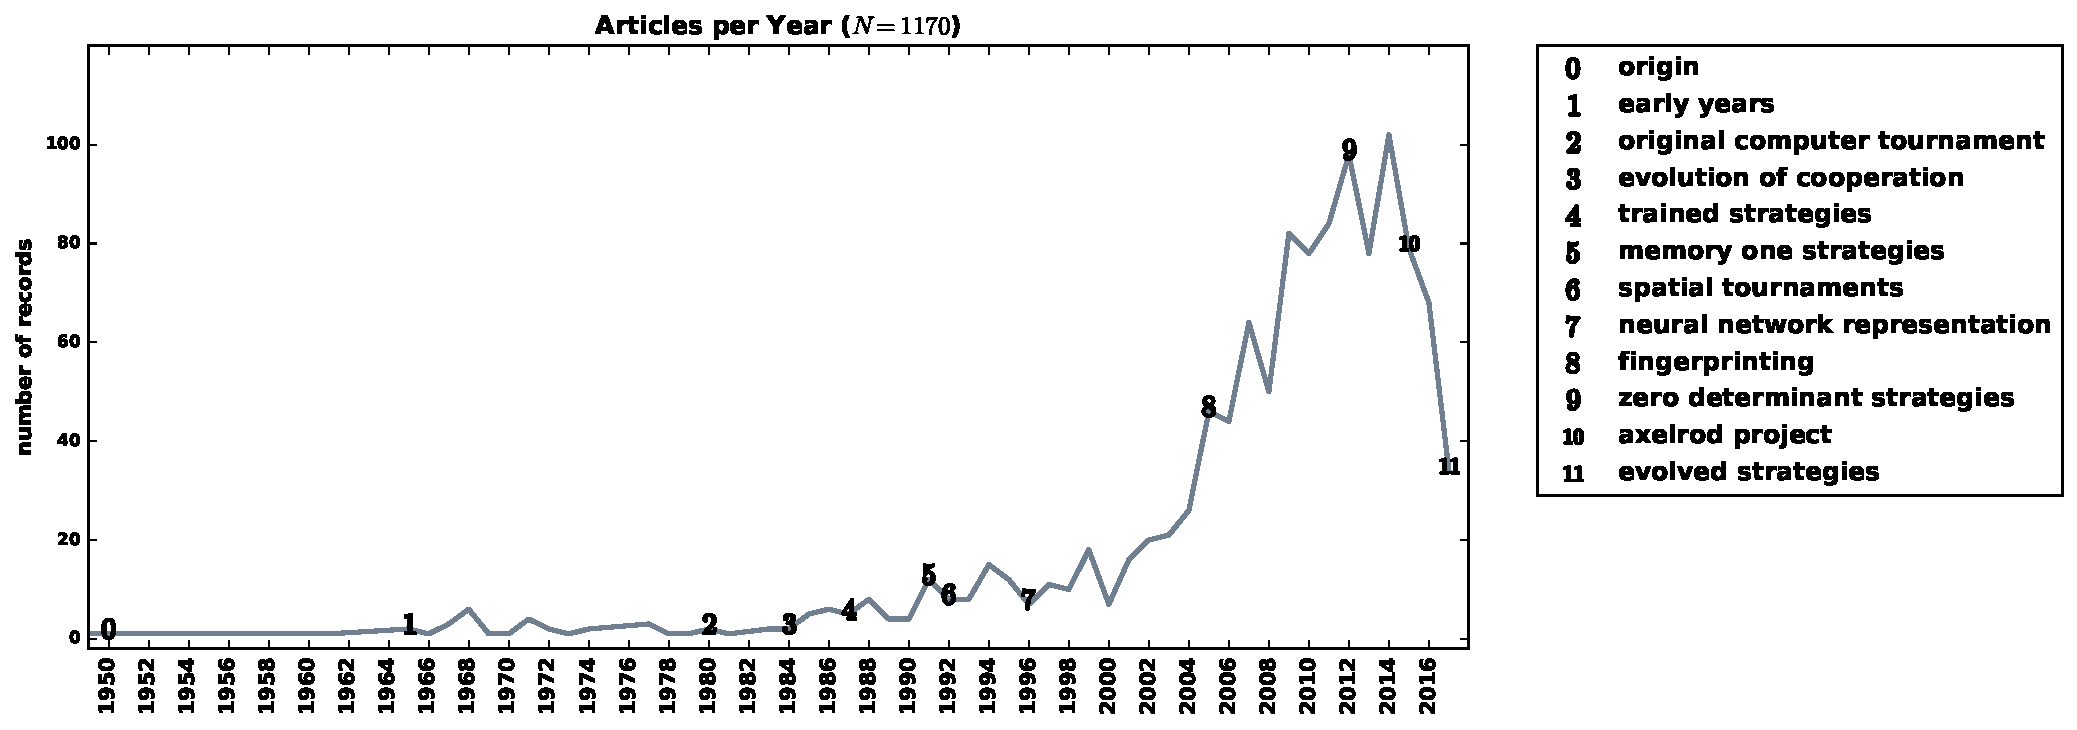
\includegraphics[width=\textwidth]{assets/images/timeline.pdf}
    \caption{\label{fig:timeline} A timeline of the prisoner's dilemma research.}
\end{figure}

\section{Timeline}\label{section:timeline}

\subsection{Origin and Primal research (1961-1972)}

The origin of the prisoner's dilemma goes back to the 1950s in early experiments
conducted in RAND~\cite{Flood1958} to test the applicability of games
described in~\cite{VonNeumann1944}. Although in~\cite{Flood1958} the two player
game was introduced the name behind the game was given later the same year.
According to~\cite{Tucker1983}, A. W. Tucker (the PhD supervisor of J. Nash),
in an attempt to delivery the game with a story during a talk used prisoners as
players and the game has been known as the prisoner's dilemma ever since~\cite{Tucker1983}.

The study of the prisoner's dilemma has attracted people from various fields
across the years. An early figure within the field is Prof A. Rapoport,
a mathematical psychologist, whose work focused on peacekeeping.
In his early work~\cite{rapoport1965} Rapoport conducted experiments using humans
to simulate a play of the prisoner's dilemma. Experimental groups were not been
used only by Rapoport but it was a common mean of studying the game
\cite{Evans1966, Gallo1968, Lutzker1961, Mack1971, Sensenig1972} and are still
being used today. %TODO reference a good article with human studies.

Those experiments explored the conditions under which altruist behaviour emerges
in human societies. Conditions such as, the gender~\cite{Evans1966,
Lutzker1961, Mack1971} of individuals, the representation of the game
\cite{Evans1966}, the distance between players~\cite{Sensenig1972}, the initial effects
\cite{Tedeschi1968} and whether the experimenter was biased~\cite{Gallo1968}.

Even though, several of these experiments were held and continuous research on
the topic was undergoing game theorists were still in disagreement about
the best way to play the game~\cite{rapoport1965}. Inspired by the work of
Rapoport and intrigued by the very same question the political scientist R.
Axelrod took upon himself to identify the dominant strategy of the prisoners dilemma.

The main difference of Axelrod's approach was that machines were going to be used
instead of humans. The issues with using humans, according to Axelrod
\cite{Axelrod2012}, was the fact that humans can act very randomly even though
the aim of the game is clear to them. Thus, Axelrod was the first researcher,
to the author's knowledge, to perform a computer tournament of the iterated
prisoner's dilemma. The work of Axelrod is considered one of the greatest
milestones within the field. The tournaments and their results are discussed in
the next sections.

\subsection{Axelrod's Tournaments (1981-1984)}\label{subsection:axelrods_tournament}

This section serves as a follow up from the earlier years of the topic and as an
introduction to the modern ways of studying the prisoner's dilemma. It is
dedicated to the computer tournaments of R. Axelrod from 1981 to 1984.

The first computer tournament was performed in 1980~\cite{Axelrod1980a}.
Several scientists were invited to submit their strategies, written in the
programming languages Fortran or Basic. There was a total number 13 submissions
made by the following researchers,

\begin{multicols}{2}
    \begin{enumerate}
        \item T Nicolaus Tideman and Paula Chieruzz;
        \item Rudy Nydegger;
        \item Bernard Grofman;
        \item Martin Shubik;
        \item Stein and Anatol Rapoport;
        \item James W Friedman;
        \item Morton Davis;
        \item Jim Graaskamp;
        \item Leslie Downing;
        \item Scott Feld;
        \item Johann Joss;
        \item Gordon Tullock;
        \item Name not given.
    \end{enumerate}
\end{multicols}

Each competed in a 200 turn match against all 13 opponents, itself and a player
that played randomly. This type of tournament is referred to as a round robin and
corresponds to a complete graph from a topological point of view. The tournament
was repeated \(5\) times to reduce variation in the results. Each participant knew
the exact length of the matches and had access to the full history of each match.
Furthermore, Axelrod performed an preliminary tournament and the results were known
to the participants. The payoff values used for~\ref{eq:the_pd_payoffs} where
\(R=3, P=1, T=5\) and \(S=0\). These values are commonly used in the literature
and unless specified will be the values used in the rest of the work described here.

The winner of the tournament was determined by the total average score and not by
the number of matches won. The strategy that was announced the winner was
submitted by Rapoport and was called \textbf{Tit For Tat}. Tit for Tat, is a
strategy that always cooperates on the first round and then mimics the opponent's
previous move.

Examples of Tit for Tat interacting for 8 turns with deterministic opponents are
given by Tables~\ref{table:tft_vs_c}, \ref{table:tft_vs_d}, \ref{table:tft_vs_a}.
The opponents are, \textbf{Cooperator} a strategy that always cooperates,
\textbf{Defector} an opponent that always defects and \textbf{Altenator} a
player who alternates between cooperating and defecting.

\begin{table}[!hbtp]
    \begin{center}
    \begin{tabular}{lcc}
        \toprule
        Turns & Tit for Tat & Cooperator\\
        \toprule
        1 & C & C \\
        2 & C & C \\
        3 & C & C \\
        4 & C & C \\
        5 & C & C \\
        6 & C & C \\
        7 & C & C \\
        8 & C & C \\
        \bottomrule
    \end{tabular}
    \caption{Tit for Tat example match of 8 turns against Cooperator}\label{table:tft_vs_c}
    \end{center}
\end{table}

\begin{table}[!hbtp]
    \begin{center}
    \begin{tabular}{lcc}
        \toprule
        Turns & Tit for Tat & Defector\\
        \toprule
        1 & C & D\\
        2 & D & D\\
        3 & D & D\\ 
        4 & D & D \\
        5 & D & D\\
        6 & D & D\\ 
        7 & D & D \\
        8 & D & D \\
        \bottomrule
    \end{tabular}
    \caption{Tit for Tat example match of 8 turns against Defector}\label{table:tft_vs_d}
\end{center}
\end{table}

\begin{table}[!hbtp]
    \begin{center}
    \begin{tabular}{lcc}
        \toprule
        Turns & Tit for Tat & Altenator\\
        \toprule
        1 & C & C \\ 
        2 & C & D \\ 
        3 & D & C \\ 
        4 & C & D \\
        5 & D & C \\ 
        6 & C & D \\ 
        7 & D & C \\ 
        8 & C & D \\
        \bottomrule
    \end{tabular}
    \caption{Tit for Tat example match of 8 turns against Altenator}\label{table:tft_vs_a}
\end{center}
\end{table}

The results of the first tournament were filled with surprises. Tit for Tat the
simplest strategy of all had won and had managed to defeat even entrants that
tried to improve on Tit for Tat after the preliminary tournament results.
Axelrod justified the success of the strategy saying that the strategy was
`nice' and `forgiving'.

The top eight ranked strategies were strategies that did no defect on the first
round, thus they were described as `nice' strategies. Compared to the rest of the
"nice" strategies, Tit for Tat had also another property. That property was
`forgiveness'. Tit for Tat punished it's opponent for a defection but just once
and then it would try to cooperate again. These two properties were described to
be the secret of success in a prisoner's dilemma tournament.

In order to further test the robustness of the results Axelrod performed a second
tournament~\cite{Axelrod1980b} later in 1980. This time a total of 63 participants
submitted strategies for the second tournament, their names were the following,

\begin{multicols}{3}
    \begin{enumerate}
        \item Gail Grisell;
        \item Harold Rabbie;
        \item James W Friedman;
        \item Abraham Getzler;
        \item Roger Hotz;
        \item George Lefevre;
        \item Nelson Weiderman;
        \item Tom Almy;
        \item Robert Adams;
        \item Herb Weiner;
        \item Otto Borufsen;
        \item R D Anderson;
        \item William Adams;
        \item Michael F McGurrin;
        \item Graham J Eatherley;
        \item Richard Hufford;
        \item George Hufford;
        \item Rob Cave;
        \item Rik Smoody;
        \item John Willaim Colbert;
        \item David A Smith;
        \item Henry Nussbacher;
        \item William H Robertson;
        \item Steve Newman;
        \item Stanley F Quayle;
        \item Rudy Nydegger;
        \item Glen Rowsam;
        \item Leslie Downing;
        \item Jim Graaskamp and Ken Katzen;
        \item Danny C Champion;
        \item Howard R Hollander;
        \item George Duisman;
        \item Brian Yamachi;
        \item Mark F Batell;
        \item Ray Mikkelson;
        \item Craig Feathers;
        \item Fransois Leyvraz;
        \item Johann Joss;
        \item Robert Pebly;
        \item James E Hall;
        \item Edward C White Jr;
        \item George Zimmerman;
        \item Edward Friedland;
        \item X	Edward Friedland;
        \item Paul D Harrington;
        \item David Gladstein;
        \item Scott Feld;
        \item Fred Mauk;
        \item Dennis Ambuehl and Kevin Hickey;
        \item Robyn M Dawes and Mark Batell;
        \item Martyn Jones;
        \item Robert A Leyland;
        \item Paul E Black;
        \item T Nicolaus Tideman and Paula Chieruzz;
        \item Robert B Falk and James M Langsted;
        \item Bernard Grofman;
        \item E E H Schurmann;
        \item Scott Appold;
        \item Gene Snodgrass;
        \item John Maynard Smith;
        \item Jonathan Pinkley;
        \item Anatol Rapoport.
    \end{enumerate}
\end{multicols}

All the participants knew the results of the previous tournament. The rules
were similar to those of the first tournament with only one exception;
the number of turns was not specified instead a fixed probability (refereed to as
`shadow of the future'~\cite{Axelrod1988}) of the game ending on the next move
was used. The fixed probability was chosen to be 0.0036 so that the expected
median length of a match would be 200 turns. The topology was of a round robin
and each pair of players was matched 5 times. The length of the matches was
determined once by drawing a random sample. Each of the five matches had a length
of 63, 77, 151 and 308.

The results of the tournament once again came as a surprise. Tit for Tat was
considered to be one of the simplest submissions in the second tournament and won
the second tournament as well.
Tit for Tat provided proof that reciprocity behaviour can allow cooperation
to emerge in the iterated prisoner's dilemma game. In~\cite{Axelrod1980a}
the main conclusions indicating strong performance was:

\begin{itemize}
    \item that it start of by cooperating
    \item it would forgive it's opponent after a defection
    \item after opponents identified that they were playing Tit for Tat choose
    to cooperate for the rest of the game.
\end{itemize}
%The strategies of the second tournament where bias due the first tournament. Discuss with V.

Another successful strategy from Axelrod's tournament that can been seen
in literature to date is \textbf{Grudger}, originally submitted by James W. Friedman.
Grudger is a strategy that will cooperate as long as the opponent does not defect.
The name Grudger was give to the strategy
in~\cite{Li2014}. Though the strategy goes by many names in the literature such as,
Spite~\cite{Beaufils1997}, Grim Trigger~\cite{Banks1990} and Grim~\cite{Van2015}.

As for the rest of the strategies, though a full explanation of all 13 submitted strategies
is given in~\cite{Axelrod1980a} the same does not hold for all 63 strategies of
the second tournament~\cite{Axelrod1980b}. The author mainly focuses on the high
ranked participants and several details for the rest strategies are left unknown.

The source code of the 63 strategies be found on Axelrod's personal
website~\cite{fortan_code}. The source code was written by Axelrod and several
other contributors. The strategies written in Basic were translated to
Fortran before the tournament. The source code includes the code only for the
strategies and not for creating and performing the tournament.Figure~\ref{fig:tit_for_tat_fortran}
serves as an example of the source code giving the code for the winning
strategy Tit for Tat. Unfortunately, the source code of the first 13 strategies
is not available, as stated in Axelrod's personal website~\cite{fortan_code}.

\begin{figure}[!hbtp]
    \centering
    \begin{minted}
        [
        autogobble=true,
        framesep=2mm,
        fontsize=\normalsize,
        ]
        {fortran}
    FUNCTION K92R(J,M,K,L,R, JA)
C BY ANATOL RAPOPORT
C TYPED BY AX 3/27/79 (SAME AS ROUND ONE TIT FOR TAT)
c replaced by actual code, Ax 7/27/93
c  T=0
c   K92R=ITFTR(J,M,K,L,T,R)
      k92r=0
      k92r = j
c test 7/30
c   write(6,77) j, k92r
c77   format(' test k92r. j,k92r: ', 2i3)
      RETURN
      END
    \end{minted}
    \caption{\label{fig:tit_for_tat_fortran} Source code for Tit for Tat in Fortran.
    Provided by~\cite{fortan_code}.}
\end{figure}

So far it has been discussed how the performance of the strategy has been tested
through tournaments against other strategies. A question remains: is the overall
success of a strategy based only on it's performance in a round robin tournament
or should it be checked through other ways as well?

Following his initial tournaments Axelrod performed an `ecological' tournament
in 1981~\cite{Axelrod1984}. Axelrod argued that some strategies are so unsuccessful
that there are very likely to be dropped in the future, while other more successful
strategies would continue in later interactions. Influenced by evolutionary biology
Axelrod introduced a way of capturing this behaviour, which included running a
series of tournaments where more successful strategies would occupy a larger part
of the environment and the less successful strategies would become less often.
This is known as an ecological tournament.

The simulation of the process, as described in~\cite{Axelrod1984}, is straightforward.
Consider matrix~\ref{eq:interaction_payoffs} which provides the expected payoff
when two individuals of different type interact. Starting with proportions of
each type in a given generation the proportions of these strategies in the next
generation is the only measure needed to be calculated. This is achieved by
calculating the weighted average of the scores of a given strategy with all
other players, where the weights are the numbers of the other strategies which
exist in the current generation. The numbers of a given strategy in the next
generation is then taken to be proportional to the product of its numbers in the
current generation and its score in the current generation.

\begin{equation} \label{eq:interaction_payoffs}
    \begin{pmatrix}
    (R=3, R=3) & (S=0, T=5) \\ (T=5, S=0) & (P=1, P=1)
    \end{pmatrix}
\end{equation}

Note the ecological tournament does not offer any evolutionary perspective.
There is no possibility of a new strategy to be introduced, there is no mutation
probability to drive the evolution. The ecological is a framework that provides
the distributions of given types over time when interacting with the population.

The set of strategies from Axelrod's second tournament was used to perform the
ecological tournament. Several interesting insights were reported,

\begin{itemize}
    \item The lowest ranking 11 strategies had fallen to half their initial size
    by the 5 generation;
    \item The middle-ranking entries managed to hold their initial size;
    \item By the \(500^{th}\) generation the only strategies that were larger than their
    initial size have been the top 11 ranked strategies;
    \item These formed 96\% of the population at that time;
    \item The rule which ranked fifth in the tournament, submitted by William Adams,
    grew to three times its original size in the population and then began to sink
    after generation 100;
    \item The rule which ranked eighth, submitted by Paul D. Harrington, and was
    the only non nice rule in the top 15, grew to four times its original size but
    began to shrink after generation 150 to reach only a third of its original
    size by the \(1000^{th}\) generation.
\end{itemize}

Overall the strategies that did rank at the top of the second tournament have
also ranked top in the ecological tournament. On the same note, the strategy that
was ranked at the top was again Tit for Tat. By the 1000th generation it was 14.5\%
of the whole population, followed by the third place rule at 13.9\% and then the
second place rue at 13.1\%, Tit for Tat was growing at .05\% per generation which
was a faster rate than any other strategy. All these ar captured in
Figure~\ref{fig:ecological.tournament}.

The ability of strategies to be favoured under natural selection and their
ability to withstand invasion from other strategies soon became a measure
of performance; refereed to as the stability of a strategy.

\begin{figure}[!hbtp]
    \centering
    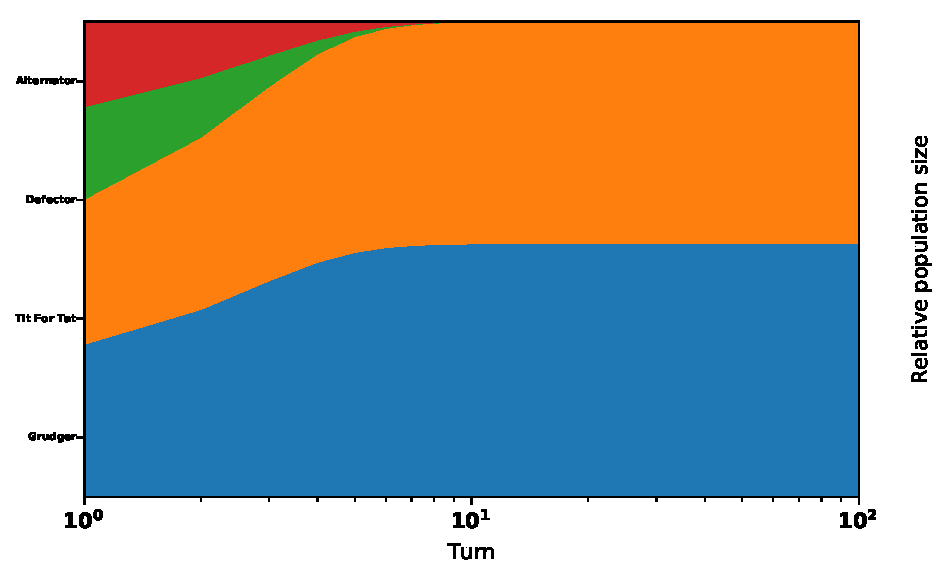
\includegraphics[width=.6\textwidth]{./assets/images/ecological.pdf}
    \caption{System evolving over time based on natural selection using
    \cite{axelrodproject}, strategies set from Axelord's second tournament.}
    \label{fig:ecological.tournament}
\end{figure}

A much more general approach was discussed in~\cite{axelrod1981}; the evolutionary
approach. Imagine a population made up of individuals where everyone follows the
same strategy, \(B\) and a single individual adopts a mutant strategy \(A\).
Strategy \(A\) is said to invade strategy \(B\) if,

\begin{equation}
V(A \mid B) > V(B \mid B)
\end{equation}
where \(V(B \mid B)\) is the expected payoff received by \(B\) against itself.

Since the strategy \(B\) is an population that interacts only with itself,
the concept of invasion is equivalent to a single mutant being able to outperform
the average population. This leads to the concept of the evolutionary approach.
Thus for a strategy to be \textbf{evolutionary stable} it must be able to
resists any invasion. There are several applications in biology for the interpretation
of this approach, for example the survival of the fitness in wildlife.

Due the large number of possible strategies in the prisoner's dilemma identifying
all the stable strategies was a difficulty task at the time. Axelrod focused
the work of~\cite{axelrod1981} in three questions,

\begin{enumerate}
    \item Under what conditions was Tit for Tat evolutionary stable?
    \item What were the necessary and sufficient conditions for any strategy to be
    evolutionary stable?
    \item Finally, in an environment where all followed a strategy of unconditional
    defection, can cooperation emerge?
\end{enumerate}

A series of theorems were presented which showed, that Tit for Tat is evolutionary
stable y if and only if it is invadable neither by Defector nor Alternator. This
is true only if the game is likely to last long enough for the retaliation
to counteract the temptation to defect, according to Axelrod. Secondly,
Defectors can withstand invasion by any strategy, as long as the players using
other strategies come one at a time. But if they come in clusters (even in rather small
clusters), the strategy could be invaded. As for the characteristics of stable
strategies, Axelrod provided a series of theorems.

\subsubsection{Response to the computer tournaments (1984-1993)}

The pioneering work of computer tournaments and the results on the reciprocal behaviour
of the prisoner's dilemma spread the knowledge of the game not only worldwide
but also across different scientific principles. The study of cooperation became
of critical interest once again. This section focuses on the immediate research
that was carried out after the initial computer tournaments.

Ecological studies that made use of Axelrod's results include the
works of~\cite{Godfray1992, Milinski1987, Wilkinson1984}, more specifically how
the successful strategy Tit for Tat can be applied in nature and wildlife.

In~\cite{Milinski1987} the behaviour of fish when confronting a potential predator
was studied. Conflicts can arise within pairs of fish in these circumstances.
Two experiments were held using a system of mirrors where sticklebacks would be
accompanied by  a cooperating companion or a defecting one. In both cases the hypothesis
that the fish would behave according to Tit for Tat and that cooperation would evolve
were supported. The works of~\cite{Godfray1992, Wilkinson1984} looked at
food sharing between vampire bats and explained behaviour based on famous at
that time tournament strategies.

Axelrod's tournaments assumed that each player has perfect information of the
opponent's actions. In real life situations this is not always the case.
Interactions often suffer from measures of uncertainty. In the original tournaments
there was no possibility of misunderstanding.

In 1985, P. Molander tested the robustness of Tit for Tat in an uncertain environment
by introducing noise~\cite{Molander1985}. Noise is a probability that that one's
move will be flipped. Molander findings stated that if two strategies playing Tit
for Tat meet in a noisy match the average payoff that a strategy will receive will
be the same as that of a Random player (with probability \(0.5\) of cooperating).

Further work on the performance of Tit for Tat in uncertain environments was
conducted, described in~\cite{Bendor1991, Godfray1992, Nowak1992}. These works
focused, similar to Molander's, focused on how the strategy suffers against itself
the most. In a noise environment, where a random defection can occur, the two
strategies would end up in an unwanted circle of defection-cooperation. In a non
noisy environment the strategies would have cooperated until the final interaction.

In~\cite{Bendor1991} a similar tournament to that of Axelrod's was performed
but this time noise was used. J. Bendor invited academics to submit strategies
to participate in the tournament. A total of thirteen strategies were used
including already existed strategies such as Tit for Tat and \textbf{Tit for Two
Tats}~\cite{Axelrod1988}. Tit for Two Tats is a variant of the classic strategy
that defects only when the opponent has defected twice in a row. The findings
of the tournaments suggested that a more forgiving strategy is needed in a noisy
environment. The winner of this tournament was a strategy called
\textbf{Nice and Forgiving}.

The work of~\cite{Nowak1992} aimed to also investigate stochastic effects.
Using an evolutionary setting of a heterogeneous population where noise is taken
into account, the space of reactive strategies was explored. Though a small fraction
of Tit for Tat players have been essential for the emergence of cooperation,
more generous strategies took over the population. This reactive strategy was
is known as \textbf{Generous Tit for Tat} and can be presented as \((0, \frac{2}{}3)\).

Reactive strategies are a subset of memory one strategies introduced in 1989~\cite{nowak1989}.
Reactive strategies are denoted by the probabilities to cooperate after an
opponent's \textbf{C} or \textbf{D} respectively. Thus, a reactive strategy only
considers the previous turn of the opponent. Memory one strategies, are a set of
strategies that consider the entire last turn of the game to decide on a next move.

Memory one strategies were also introduced by M. Nowak in 1990~\cite{Nowak1990}.
Depending on the simultaneous moves of two players the states of the game,
when only the previous round is considered, a state where both cooperated,
both defected or either of them defected. These states are represented as
\(CC, CD, DC, DD\). A memory one strategy can be written as the probability of
cooperating after each of these states. Thus as a vector of four probabilities
\(p\) where \( p = (p_1, p_2, p_3, p_4) \in\mathbb{R}_{[0,1]}^{4} \).
Reactive strategies are just a constrained version of memory one strategies where
\(p_1=p_3\) and \(p_2=p_1\).

The above formulation offered a new framework of studying strategies. Consider
that two memory one strategies are in a game of the prisoner's dilemma. Their
interaction can be written as the following markov chain,

\begin{equation}\label{eq:markov_matrix}
    M =
\begin{bmatrix}
    p_{1} q_{1} & p_{1} (- q_{1} + 1) & q_{1} (- p_{1} + 1) & (- p_{1} + 1) (- q_{1} + 1)
    \\
    p_{2} q_{3} & p_{2} (- q_{3} + 1) & q_{3} (- p_{2} + 1) & (- p_{2} + 1) (- q_{3} + 1)
    \\
    p_{3} q_{2} & p_{3} (- q_{2} + 1) & q_{2} (- p_{3} + 1) & (- p_{3} + 1) (- q_{2} + 1)
    \\
    p_{4} q_{4} & p_{4} (- q_{4} + 1) & q_{4} (- p_{4} + 1) & (- p_{4} + 1) (- q_{4} + 1)
    \\
\end{bmatrix}
\end{equation}

where the opponent is denoted as \(q=(q_1, q_2, q_3, q_4) \in\mathbb{R}_{[0,1]}^{4}\).
The expected state that two opponents will end up can be estimated by calculating
the steady states of the markov chain.

Nowak, as described, studied the reactive but also the memory one strategies
space and introduced several other strategies, among them the most popular was
\textbf{Pavlov}. Pavlov is a strategy with the tolerance of Generous Tit for Tat
but also the capability of resisting and invading an all-out cooperators population.
The strategy is based on the fundamental behavioural mechanism win-stay,
lose-shift. It starts off with a cooperation and then repeats it's previous move
only if it was awarder with a payoff of \(R\) or \(T\). Otherwise it shifts
it's last move.

A number of researchers searched for new strategies. Such strategies have been,
\textbf{Handshake}~\cite{Robson1989} and \textbf{Gradual}~\cite{Beaufils1997}.
Presented in 1989 and 1997 respectively.Handshake was developed using an
evolutionary tournament, where Gradual performance was tested in both a round-robin
tournament and ecological simulation.

Handshake is a strategy that starts with cooperation, defection. If the opponent
plays in a similar way then it will cooperate forever, otherwise it will defect
forever. Gradual starts off by cooperating, then after the first defection of the
other player, it defects one time and cooperates twice. After the second defection
of the opponent, it defects two times and cooperates twice. After the \(n^{th}\)
defection it reacts with \(n\) consecutive defections and then two cooperations.

Another measure of uncertainty is that of mis perception. Though noise will flip
a player's action it will be recorded correctly in the history. Mis perception is
the probability that the opponent's current move is flipped before being recorded
\cite{Hoffmann1998}.

\subsection{Evolutionary Dynamics (1987-1999)}

Determining the evolutionary stability of strategies for the iterated prisoner's
dilemma as we discussed is not an easy task. Methods can be use to deal with
the difficulty. In~~\cite{Boyd1987} the author restricted the possible strategies
that could be adopted to a relatively narrow set and resulted that no pure strategy
is evolutionary stable, including Tit for Tat. Arguing with the results presented
in~\cite{axelrod1981}. The list of strategies used included strategies such as
Defector and \textbf{Suspicious Tit for Tat}, a strategy that plays
Tit for Tat but starts by defecting.

The results were questioned by~\cite{May1987}, stating that much was still no fully
explored and more research had to be put into the results. Farrel and Ware in
1989~\cite{Farrell1989} extended the result to include finite mixture of pure
and mixtures of Tit For \(n\) Tats as well. On the same year the work of~\cite{Boyd1989}
looking again at a narrow set of strategies extended their results to
noisy environments.

Evolutionary dynamics have been highly useful in the research of the prisoner's
dilemma. In~\cite{Axelrod1987}, an evolutionary process, called the genetic
algorithm, was used to discover effective strategies. The author introduced
lookup tables as a mean of representing a strategy in a gene format. A lookup
table is a set of deterministic responses based on the opponents \(m\) last
moves; \cite{Axelrod1987} considered \(m=3\).

An extension to the natural selection was introduced in the 1992~\cite{Nowak1992b},
recommending a different type of topology. A population of two deterministic
strategies, Defector and Cooperator, were placed on a a two dimensional square array
where the individuals could interact only with the immediate neighbours.
The number of immediate neighbours could be either, fourth, six or eight. As
shown in Figure~\ref{fig:topologies}. The authors claimed that the essential
results remain true of all topologies; the results also hold whether self interactions
are taken into account.

Thus each cell of the lattice is occupied by a Cooperator or a Defector. At
each generation step each cell owner interacts with its immediate neighbours.
The score of each player is calculated as the sum of all the scores the player
achieved at each generation. At the start of the next generation, each lattice
cell is occupied by the player with the highest score among the previous owner
and the immediate neighbours. This topology is refereed to as spatial topology.

Nowak studied the population dynamics as a function of the temptation payoff.
It was shown that for different values of the temptation payoff, cooperators
and defectors could persist together.

\begin{figure}[!hbtp]
\centering
    \begin{subfigure}{.25\textwidth}
        \hspace{.8cm}
        \includestandalone[width=0.6\textwidth]{assets/tex/neighb_four}
    \end{subfigure}
    \begin{subfigure}{.25\textwidth}\centering
        \includestandalone[width=0.6\textwidth]{assets/tex/neighb_eight}
     \end{subfigure}
     \begin{subfigure}{.25\textwidth}\centering
        \includestandalone[width=0.6\textwidth]{assets/tex/neighb_six}
     \end{subfigure}
    \begin{subfigure}{.25\textwidth}
        \includestandalone[width=\textwidth]{assets/tex/square_lattice}
    \end{subfigure}
    \begin{subfigure}{.25\textwidth}\centering
        \includestandalone[width=\textwidth]{assets/tex/square_lattice_eight}
     \end{subfigure}
     \begin{subfigure}{.25\textwidth}\centering
        \includestandalone[width=\textwidth]{assets/tex/hexagonal_lattice}
     \end{subfigure}
     \caption{Spatial neighbourhoods}\label{fig:topologies}
    \end{figure}

This work dealt with dealt with symmetric spatial lattices in two dimensions,
deterministic winning and discrete time. The authors in later work~\cite{nowak1994},
that the results remain valid in more realistic situations. Such as situations
where the spatial distributions of cells are random in two or three dimensions,
and where winning is partly probabilistic.

\subsection{Modern approaches (1995-2015)}\label{section:modern_approaches}

A number of aspects discussed in the previous sections such as round robin
tournaments, evolutionary tournaments, training of strategies and noise environments
soon became standard means of studying the iterated prisoner's dilemma. In this
section we review a number of computer tournament that used these methods
and introduced a number of findings that made an impact in the literature.

Initially in 1995 a combination of tournament studies, ecological simulations
and theoretical analysis was used in~\cite{Wu1995} to demonstrate approaches to
copy with noise. These included generosity, contrition and win-stay, lose-shift
by respectively using the strategies Generous Tit for Tat, \textbf{Contrite Tit for Tat}
and Pavlov. A fourth strategy was also analysed \textbf{Generous Pavlov}.
A strategy that acts like Palvov but cooperates 10\% of the time when it would
defect otherwise.

- \textbf{Adaptive Tit for Tat}~\cite{tzafestas-2000a}.

Less generous variants also made an appearance~\cite{Hilde2013}.
\textbf{Anti Tit for Tat}, is a strategy that plays the opposite of the opponents
previous move. Another limitation of the strategy was discussed in~\cite{Wolfgang2006}.
Tit for Tat was proven to hit a loop between cooperation and defection.
\textbf{Omega Tit For Tat} was introduced and was a strategy capable of avoiding
such problem~\cite{Wolfgang2006}.

In 2011 the authors of~\cite{Li2011} performed their own tournament where
several interesting strategies made an appearance.

\begin{itemize}
    \item \textbf{Periodic player CCD}, plays \textbf{C}, \textbf{C}, \textbf{D}
    periodically. Note that variations of a period player also make appearance
    in the article but will not be listed here.
    \item \textbf{Prober}, starts with the pattern \textbf{D}, \textbf{C}, \textbf{C}
     and then defects if the opponent has cooperated in the second and third move;
     otherwise, it play as Tit for Tat.
    \item \textbf{Reverse Pavlov}, a strategy that does the reverse of Pavlov.
\end{itemize}

In earlier work the same author introduced a strategy called \textbf{APavlov},
which stands for adaptive Pavlov~\cite{Li2007}. The strategy attempts to
classify the opponent as one of the following strategies, All Cooperator,
All Defector, Pavlov, Random or \textbf{PavlovD}. PavlovD, is just Pavlov
but it starts the game with a \textbf{D}. Once Adaptive Pavlov has classified
the opponent plays to maximize it's payoff.

Evolutionary dynamics and optimization methods are used with different representation
methods in order to discover new optimized strategies. Include lookup tables
\cite{Axelrod1987, Lindgren1994}, artificial neural networks~\cite{Fogel1996,
Lee2015} and finite state machines~\cite{Miller1996, Rubinstein1986}.

Strategies based on finite state machines are described by the number of states.
The strategy selects the next action in each round based on the current state
and the opponent's last move, transitioning to a new state each time. Figure~\ref{fig:tit_for_tat_fsm},
illustrates the finite state representation of Tit For Tat.

\begin{figure}[!hbtp]
    \centering
    \includestandalone[width=.3\textwidth]{./assets/tex/tit_for_tat_fsm}
    \caption{Finite state machine representation of Tit for Tat.}
    \label{fig:tit_for_tat_fsm}
\end{figure}

In~\cite{Ashlock2006b} the author presented two new strategies that have
been trained using a finite state machine representation. They are called,
\textbf{Fortress3} and \textbf{Fortress4}. Figure~\ref{fig:fortress3_and_4}
illustrates their diagrammatic representation where the transition arrows are
labelled \textit{O/P} where \textit{O} is the opponent's last action and \textit{P}
is the player's response.

\begin{figure}[!hbtp]
\centering
    \begin{subfigure}{.4\textwidth}
        \includestandalone[width=\textwidth]{assets/tex/fortress_3}
    \end{subfigure}
    \begin{subfigure}{.4\textwidth}\centering
        \includestandalone[width=\textwidth]{assets/tex/fortress_4}
     \end{subfigure}
     \caption{Representations of Fortress 3 and Fortress 4. Note that the
     strategy's first move, enters state 1, is defection for both strategies.}
     \label{fig:fortress3_and_4}
\end{figure}

Optimisation methods will return a spectrum of strategies. In order to distinguish
the strategies and assuring that they are indeed different \cite{Ashlock2005}
introduced a method called fingerprinting.

The method of fingerprinting is a technique for generating a functional signature for a
strategy~\cite{Ashlock2008}. This is achieved by computing the score of a strategy
against a spectrum of opponents. The basic method is to play the strategy
against a probe strategy with varying noise parameters. In~\cite{Ashlock2005}
Tit for Tat is used as the probe strategy. Fingerprint functions
can then be compared to allow for easier identification of similar strategies.
In Figure~\ref{fig:fingerprinting} an example of Pavlov's fingerprint is given.
Fingerprinting has been studied in depth in~\cite{Ashlock2008, Ashlock2009,
Ashlock2010, Ashlock2006a}.

\begin{figure}[!hbtp]
    \centering
    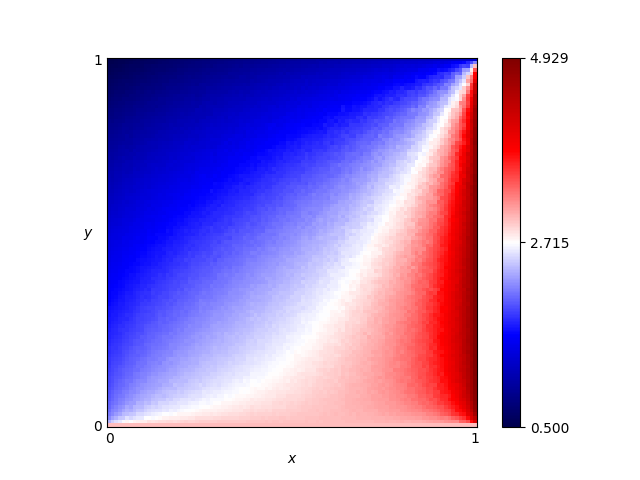
\includegraphics[height=.3\textheight]{./assets/images/Win-Stay_Lose-Shift.png}
    \caption{Pavlov fingerprinting with Tit for Tat used as the probe strategy.
    Figure was generated using~\cite{axelrodproject}.}
    \label{fig:fingerprinting}
\end{figure}

Due the nature of the research several pieces of software are starting to appear,
this includes a library called PRISON~\cite{prison}. PRISON is written in the
programming language Java and it has been used by it's authors in several
publications. The project includes a good number of strategies from the
literature but unfortunately the last update of the project dates back in 2004.

\subsection{Zero determinant (2012 - 2015)}

Following Section~\ref{section:modern_approaches}, this section is a review
of an important set of strategies, the zero determinant.

In~\cite{Press2012}, a new set of memory one strategies were introduced, called
\textbf{zero determinant (ZD)} strategies. The ZD strategies,
manage to force a linear relationship between the score of the strategy
and the opponent. Press and Dyson, prove their concept of the ZD strategies
and claim that a ZD strategy can outperform any given opponent.

The ZD strategies have attracted a lot of attention. It was stated that
``Press and Dyson have fundamentally changed the viewpoint on the Prisoner's
Dilemma''~\cite{Stewart2012}. In~\cite{Stewart2012}, a new tournament was
performed including ZD strategies and a new set of ZD
strategies the \textbf{Generous ZD}. Even so, ZD and memory one strategies have
also received criticism. In~\cite{Lee2015}, the `memory of a strategy does
not matter' statement was questioned. A set of more complex strategies,
strategies that take in account the entire history set of the game, were
trained and proven to be more stable than ZD strategies.

\subsection{Contemporary period (2015 - 2017)}

Following a discussion on research of short memory strategies this section
reviews recent work done in complex strategies. As well as a discussion of
new software and how modern approaches allows us to now revisit several pieces of
work produced in the past.

Modern approaches of artificial neural networks and machine learning are now used
in the field.  A number of strategies based on artificial neural networks are
introduced by~\cite{Knight2017}. Artificial neural networks provide a mapping
function to an action based on a selection of features computed from the history
of play.

These strategies are refereed to as \textbf{EvovlvedANN} strategies and are
based on a pre-trained neural network with the following features,

\begin{multicols}{2}
    \begin{itemize}
        \item Opponent's first move is C
        \item Opponent's first move is D
        \item Opponent's second move is C
        \item Opponent's second move is D
        \item Player's previous move is C
        \item Player's previous move is D
        \item Player's second previous move is C
        \item Player's second previous move is D
        \item Opponent's previous move is C
        \item Opponent's previous move is D
        \item Opponent's second previous move is C
        \item Opponent's second previous move is D
        \item Total opponent cooperations
        \item Total opponent defections
        \item Total player cooperations
        \item Total player defections
        \item Round number
    \end{itemize}
\end{multicols}

A representation of \textbf{EvovlvedANN 5} is given in Figure~\ref{fig:ann_5_neural}.
The inputs of the neural network are the 17 features as listed above. Number 5
reefers to the size of the hidden layer.

\begin{figure}[!hbtp]
    \centering
    \includestandalone[width=.5\textwidth]{./assets/tex/ann_5_neural}
    \caption{Neural network representation of EvovlvedANN 5.}
    \label{fig:ann_5_neural}
\end{figure}

In~\cite{Knight2017}, these representing methods are refereed to as archetypes.
Finite state machines and artificial neural networks are included in the
work but also new archetypes are introduced, such as hidden Markov models. A variant
of a finite state machine that use probabilistic transitions based on the prior
round of play to other states and cooperate or defect with various probabilities
at each state. Finite state machines and hidden Markov models
based strategies are characterized
by the number of states. Similarly, artificial neural networks based players
are characterized by the size of the hidden layer and number of input features.

Additionally a variant of a look up table is also presented called the lookerup
archetype. The lookerup archetype responses based on the opponent's first \(n_1\)
moves, the opponent's last \(m_1\) moves, and the players last \(m_2\) moves.
Taking into account the initial move of the opponent can give many insights.
For it is the only move a strategy is truly itself without being affected by
the other player. As a reminder, Axelrod in his work
highlighted the importance of the initial move and believed that it was one
of the secrets of success of the strategy Tit for Tat.

Finally, a new archetype called the Gambler is also introduced, which is a
stochastic variant of the lookerup archetype.

Archetypes are used with evolutionary algorithms to train set of
new strategies. The evolutionary algorithm used in both~\cite{Axelrod1987,
Gaudesi2016} is called genetic algorithm. Other algorithms including particle
swarm optimization have been used in research of the most dominant strategy
\cite{Franken2005}.

In~\cite{Knight2017} the approach in used to introduce as stated
by the authors the best performing strategies for the iterated prisoner's dilemma.
These strategies will be refereed  as \textbf{Evolved} strategies.
Several successful new strategies are,

\begin{itemize}
    \item \textbf{EvolvedLookerUp2\_2\_2} a looker up strategy trained with a
    genetic algorithm; EvolvedLookerUp2\_2\_2 responses based on the opponent's
    2 first and last moves and the player's 2 last moves. Thus \(n_1=2, m_1=2\)
    and \(m_2=2\).
    \item \textbf{Evolved HMM 5} a 5 states hidden markov model trained with a genetic
    algorithm;
    \item \textbf{Evolved FSM 16} a 16 state machine trained with a genetic
    algorithm;
    \item Finally \textbf{PSO Gambler 2 2 2} a looker up strategy trained with
    a particle swarm algorithm, where \(n_1=2, m_1=2\) and \(m_2=2\).
\end{itemize}

Though several papers have claimed before to have discovered the dominant
strategies for the game the work of \cite{Knight2017} is promising.
This is due the fact that the introduced strategies have been trained using
different types of evolutionary algorithms in a pool of 176 well known
strategies for the literature. Including all the strategies that have been
discussed in this section.

This was made possible due an open source  library, called the Axelrod project
\cite{axelrodproject}. The project is written in the programming language
Python, it is accessible and open source. To date the list of strategies implemented
within the library exceed the 200. The project has been used in several
publications including~\cite{Knight2017} and a paper describing it and
it's capabilities was published in 2016~\cite{Knight2016}. The source code
for Tit for Tat as implement within the library is shown in Figure
\ref{fig:tit_for_tat_axelrod}. Furthermore, performing a tournament
with a selection of strategies is possible in five lines of code, shown in
Figure~\ref{fig:tournament_code}.

\begin{figure}[!hbtp]
    \centering
    \begin{minted}
        [
        autogobble=true,
        framesep=2mm,
        fontsize=\normalsize,
        ]
        {python}
def strategy(self, opponent: Player) -> Action:
    """This is the actual strategy"""
    # First move
    if not self.history:
        return C
    # React to the opponent's last move
    if opponent.history[-1] == D:
        return D
    return C
    \end{minted}
    \caption{\label{fig:tit_for_tat_axelrod} Source code for Tit for Tat in Python
    as implemented in Axelrod Python library~\cite{axelrodproject}}.
\end{figure}

\begin{figure}[!hbtp]
    \centering
    \begin{minted}
        [
        autogobble=true,
        framesep=2mm,
        fontsize=\normalsize,
        ]
        {python}
>>> import axelrod as axl
>>> players = (axl.Cooperator(), axl.Defector(), axl.TitForTat(), axl.Grudger())
>>> tournament = axl.Tournament(players)
>>> results = tournament.play()
>>> results.ranked_names
['Defector', 'Tit For Tat', 'Grudger', 'Cooperator']
    \end{minted}
    \caption{\label{fig:tournament_code} Performing a computer tournament
    using~\cite{axelrodproject}.}
\end{figure}

Software has a crucial role in research. Well written and maintained software
allows the reproducibility of prior work and can accelerate findings within the
field. The field of the iterated prisoner's dilemma has suffered the consequences
of poor research software. As stated above the source code of the initial
computer tournament is not retrievable. Several of the strategies that competed
in the tournament are not given a full explanation of how the decided on their
next move. In terms of best practice and reproducibility the Axelrod library
is the lead software in the field.

Other recent projects include~\cite{pd_trust, pd_game}, both are education
platforms and not research tools. In~\cite{pd_trust}, several concepts such as
the iterated game, computer tournaments and evolutionary dynamics are introduced
through a user interface game. Project~\cite{pd_game} offers a big collection of
strategies and allows the user to try several match and tournaments configurations.
Such as noise.

In~\cite{Rapoport2015}, the authors claim that they have managed to
re-run the first tournament that Axelrod performed. They tried to push his work
further by altering aspects such as, the format of the tournament, the objective
and the population. One of the authors claimed to have been a contributor
to the first tournaments, which would explain how it was managed to reproduce
the tournament.

\subsubsection{Biological Applications}
%TODO include the cancer studies.
\begin{itemize}
    \item \cite{Turner1999} uses evolutionary game theory to study the spread of
    virus.
    \item \cite{Douglas2011} a shout for his work, using tit for tat to study cells.
\end{itemize}

\section{Analysis}\label{section:analysis}

In this section we will focus on the analysis of the study of the prisoner's dilemma
using a large dataset of articles. This data set will be used to ascertain the level
of collaborative nature of the field and identify influencers. This will be done
relative to:

\begin{itemize}
    \item Other sub fields of game theory: the price of anarchy~\cite{roughgarden2005}
    and auction games~\cite{menezes2005}.
    \item A temporal analysis.
\end{itemize}

\subsection{Data Collection}

Before analysing our data this subsection will describe the data collection
process.

Academic articles are accessible through scholarly databases and collections of
academic journals. Several databases and collections today offer access through
an open application protocol interface (API). An API allows users to talk
directly to the database by skipping the user interface side of a journal.
Interacting with an API has two phases:

\begin{itemize}
    \item requesting;
    \item receiving;
\end{itemize}

The request phase includes composing a url with the request. For example:

\begin{figure}[!hbtp]
    \centering
    \begin{minted}
        [
        autogobble=true,
        framesep=2mm,
        fontsize=\normalsize,
        ]
        {xml}
        http://export.arxiv.org/api/query?search_query=abs:prisoner's dilemma&max_results=1
    \end{minted}
    \caption{\label{fig:request_message} A request message for the arXiv API.}
\end{figure}

We can see in Figure~\ref{fig:request_message}, the first part of the message
indicates that we are sending a request to the arXiv~\cite{mckiernan2000} API
and the second part contains the search argument, in our example we want a single
article that the word `prisoners dilemma' exists within it's title.
This format of the request message will be different from API to API.

The second phase is receiving. This includes receiving a number of raw
metadata of articles that satisfies the requesting message. The raw metadata are
commonly received in an xml or json format~\cite{nurseitov2009}. Similarly to
the request message the structure of the received data differs from journal to journal.

This data collection is crucial to this study, to ensure that this study can be
reproduced all code used to query the different APIs has been packaged and is
available online~\cite{nikoleta_2017}. This software could be used for any type of project
similar to the one described here, documentation for it is available at
\url{http://arcas.readthedocs.io/en/latest/}.

Data was collected from the following sources,

\begin{enumerate}
        \item arXiv~\cite{mckiernan2000};
        \item PLOS~\cite{plos_one};
        \item IEEE;
        \item Nature;
        \item Springer.
\end{enumerate}

These are four prominent journals in the field as well as the arXiv~\cite{mckiernan2000}
pre print server. In the case of an article being both in a journal and the arXiv,
only the journal version was considered.

In the work described here, a series of keywords were used to identify relevant
articles. Articles for which these keywords were in the title or the abstract
are included in the analysis. A list of the keywords that were used are
shown in Table~\ref{table:search_keywords}.

\begin{table}[!hbtp]
    \begin{center}
        \begin{tabular}{lll}
            \toprule
             & Keywords & \\
            \midrule
             1 &  prisoner's dilemma & \\
             2 &  prisoners dilemma  & \\
             3 &  prisoners evolution & \\
             4 &  prisoner game theory & \\
             5 &  R Axelrod & \\
             6 &  memory one strategy & \\
             7 &  tit-for-tat & \\
             8 &  tit for tata & \\
             9 &  zero determinant strategies & \\
            \bottomrule
        \end{tabular}
    \end{center}
    \caption{Keywords used in searching for articles.}
    \label{table:search_keywords}
\end{table}

For each article~\cite{} collects data with the features shown in Table~\ref{table:arcas_results}.
Note that the plain text of the article is not collected, just the metadata. The
data is archived and available at. %TODO: archive data
In this work only the features of Table~\ref{table:result_set} are used.

\begin{table}[!hbtp]
    \begin{center}
    \resizebox{0.9\linewidth}{!}{\arraycolsep=2.5pt%
        \begin{tabular}{lll}
            \toprule
             & Result name & Explanation \\
             \midrule
             1 & Abstract & The abstract of the article.\\ 
             2 & Author & A single entity of an author from the list of
             authors of the respective article.\\ 
             3 & Date & Year of publication.\\ 
             4 & Journal & Journal of publication.\\ 
             5 & Key & A generated key containing an authors name and
             publication year (ex. Glynatsi2017).\\ 
             6 & Keyword & A single entity of a keyword assigned to the article
             by the given journal.\\ 
             7 & Labels & A single entity of labels assigned to the article
             manual by us.\\ 
             8 & Pages & Pages of publication.\\ 
             9 & Provenance & Scholarly database for where the article was
             collected.\\ 
             10 & Score & Score given to article by the given journal.\\ 
             11 & Title & Title of article.\\ 
             12 & Unique key &  A unique key. \\ 
            \bottomrule
        \end{tabular}}
    \end{center}
    \caption{Metadata for each entry/article.}
    \label{table:arcas_results}
\end{table}

\begin{table}[!hbtp]
    \begin{center}
        \begin{tabular}{lll}
            \toprule
             & Result name & Explanation \\
             \midrule
             1 & Abstract & The abstract of the article.\\ 
             2 & Author & A single entity of an author from the list of
             authors of the respective article.\\ 
             3 & Date & Year of publication.\\ 
             4 & Journal & Journal of publication.\\ 
             5 & Provenance & Scholarly database for where the article was
             collected.\\ 
             6 & Title & Title of article.\\ 
            \bottomrule
        \end{tabular}
    \end{center}
    \caption{Structure of data set. Contained results.}
    \label{table:result_set}
\end{table}

\subsection{Preliminary Analysis}

The data set~\cite{} consists of \totalarticles articles. Although only
%TODO add reference to archived dataset
\uniquetitles are unique titles. This is because a total of \numberofduplicates
articles have been collected from more than just one source. All
\numberofduplicates duplicates are from the pre print server arXiv and are
dropped for the analysis, thus hereupon we consider \uniquetitles unique article
entries. Note that not all articles were collected from the aforementioned APIs:
\manual were manually added to the dataset throughout the writing of
Section~\ref{section:timeline}. The details of how many papers came from
each source are given in Table~\ref{table:provenance}.

\begin{table}[!hbtp]
    \begin{center}
    \begin{tabular}{lrr}
\toprule
{} &  \# of Articles &  Percentage \\
provenance &                &             \\
\midrule
Manual     &             89 &        2.92 \\
IEEE       &            295 &        9.67 \\
Springer   &            458 &       15.01 \\
PLOS       &            482 &       15.79 \\
Nature     &            673 &       22.05 \\
arXiv      &           1055 &       34.57 \\
\bottomrule
\end{tabular}

    \end{center}
    \caption{Keywords used in searching for articles.}
    \label{table:provenance}
\end{table}

The oldest article was published in 1944 and the most recent one in 2017. Note
that the last time data were collected was on December 2017.
% TODO Ensure this stay accurate
The cumulative provenance of articles over time is illustrated
in Figure~\ref{fig:provenance}. This allow us to view the significance of each
journal's contribution to the field over the years as well as when the prisoner's
dilemma fitted the scope of each journal.

Springer and IEEE are the two journals that have been publishing papers on the
topic for the longest time. The first papers respectively are~\cite{Evans1966} in
1966 and~\cite{4045089} in 1973.
% TODO Add the references
% TODO POSSIBLY add sentence about each (do they correspond to something worth
% mentioning in the timeline? )
It can been seen that IEEE contributed more than 10 articles per year after 2002.
Similarly, arXiv contributes with a large number of papers with an increasing trend
after 2000. In 1991 the preprint server arXiv was lanced and the first article on
the prisoner's dilemma was published in 1993~\cite{Huberman1993}.
% TODO Add frame of reference about when the arXiv started. (Read those two
% references about the arxiv)
% TODO Invesitage if there was a rise of computer scientific journals in 2000.
% And see if the following should be modified:
%This increase could be explained due to ...
%from Section~\ref{section:timeline}, the `Modern Area' started near the 2000s
%where now the study of the prisoner's dilemma is associated with computer science.
PLOS journal was launched in 2000 and it can been seen that accepted it's first
% TODO Is there a good reference describing PLOS's philosophy? Can this be
% somewhat related to the delay in the first submission to PLOS? No matter what,
% this needs more.
publication on the topic in 2006~\cite{0020178}. Finally Nature has a few publications over the
years. Nature was one of the early destinations for publications following the
pioneering paper by Axelrod~\cite{Axelrod1984}. The first paper published was
\cite{Milinski1987} which studied the applications of Tit for Tat in nature
using sticklebacks. Another leader in the field: Nowak (mentioned in Section~\ref{section:timeline}
has published various papers in Nature~\cite{Nowak1993, Nowak1992}.

To investigate the rates of publications of each journal an exponential function
of the structure, \(a \epsilon^{b \times x}\), was fitted in each journal
provenance set. Table~\ref{table:exponential_coefficients} summarises the best coefficients based on a non
linear least square errors.

\begin{table}[!hbtp]
    \begin{center}
    \begin{tabular}{lrr}
\toprule
journal &    $a$ &   $b$ \\
\midrule
PLOS &  4.796 &  0.025 \\
Nature &  0.883 &  0.034 \\
Springer &  1.925 &  0.039 \\
IEEE &  0.889 &  0.070 \\
arXiv &  5.911 &  0.081 \\
\bottomrule
\end{tabular}

    \end{center}
    \caption{Coefficients for fitted exponential curve to provenance data.}
    \label{table:exponential_coefficients}
\end{table}

% TODO Investigate rates of increase of journal.
% Explain momentum.
% Find curves of best fit: fit line, polynomial and exponential.
% TODO Include a table of these curves of best fit and a discussion.

\begin{figure}[!hbtp]
    \centering
    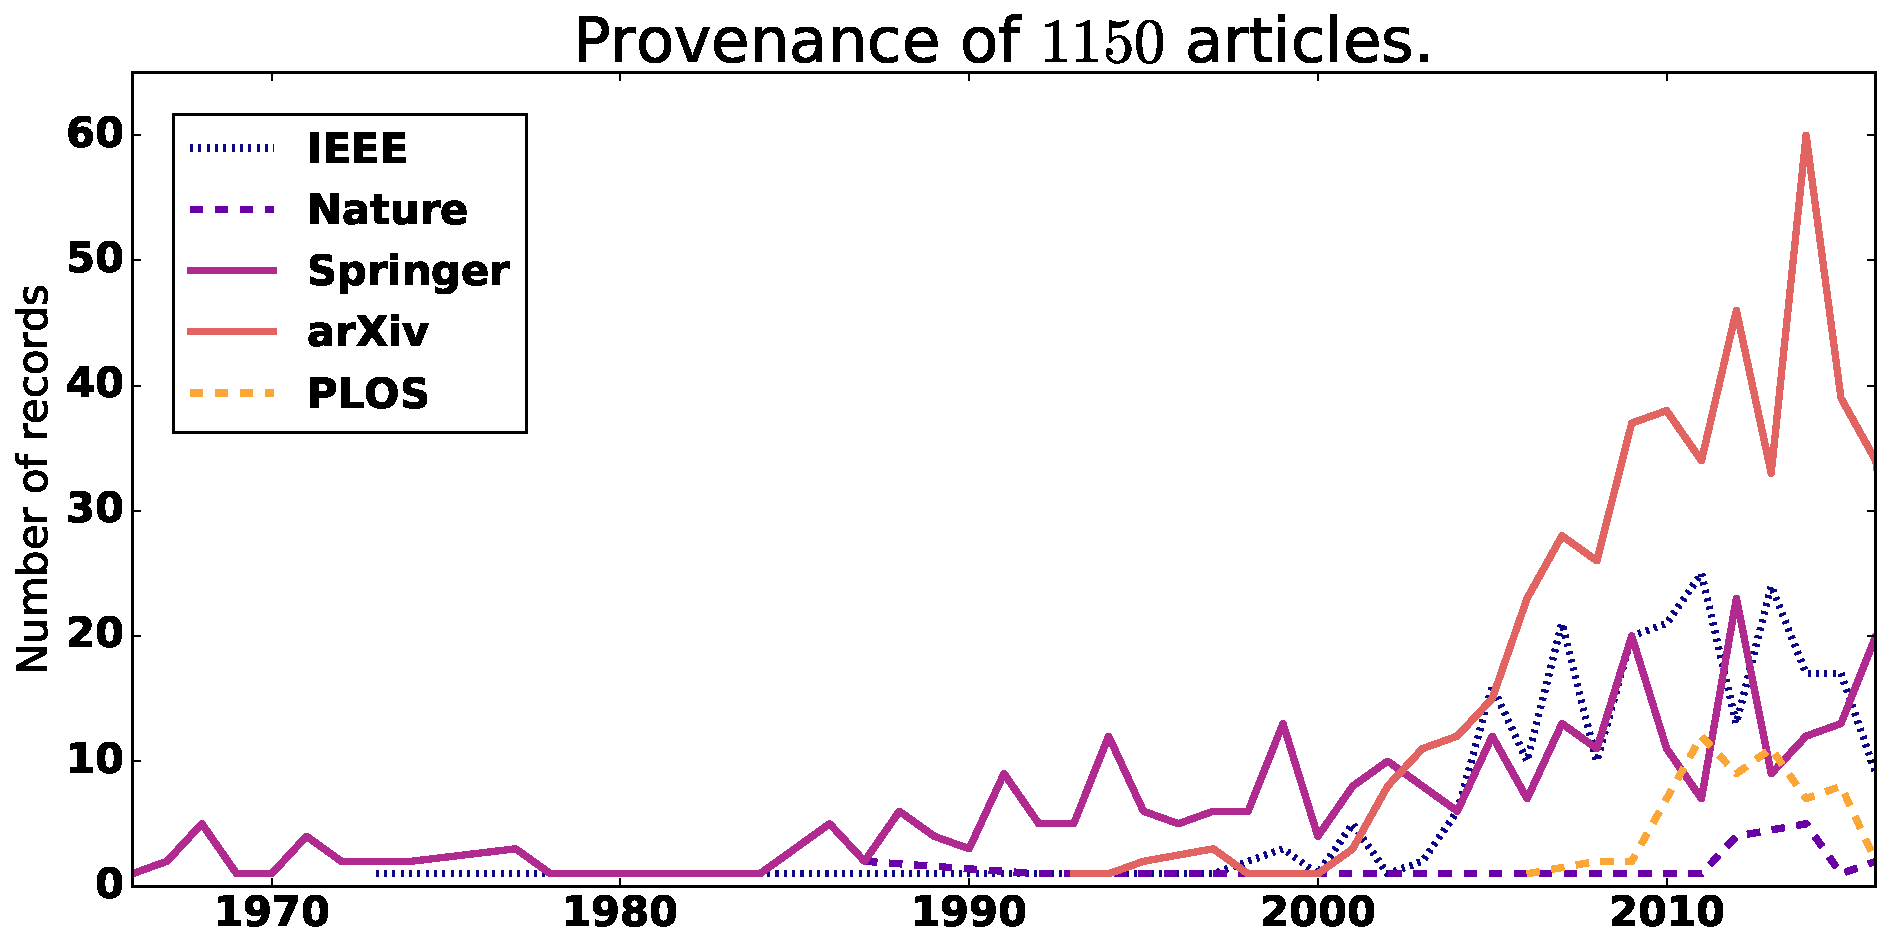
\includegraphics[width=.6\textwidth]{./assets/images/provenance.pdf}
    \caption{Provenance of articles.}
    \label{fig:provenance}
\end{figure}

Our data set contains \uniquetitles articles collected since 1944 from a variety
of sources. The overall rate at which papers have been written is calculated
as \(rate = \frac{present}{past}^{\frac{1}{n}} - 1\). The overall rate is at 6.68
percent.
% TODO summarise main findings.
In the following section we explore
the authors of the papers and their connections to one another.

\subsection{Co authorship}

% TODO Describe some works that look at literature graphs (these typically look
% at citation graphs)
% TODO Describe how these are often used to measure influence however (mention
% that blog post) influence does not correspond to citation.
% TODO Define the co author network as a weight graph G =...
% TODO Possibly include subgraphs as examples.

Measuring academic collaborations and influences is not always trivial. Many
academics tend to consider citations as a measure of how could a research project
is. According to a blog post~\cite{nature_blog} written by Nature in 2017,
depending on citation could be misleading. This is because:

\begin{itemize}
    \item The true number of citations can not be known. Citations can be missed
    due data entry errors or typos in a journal.
    \item Academics are influenced by many more papers than they actually cite.
    \item Several citations are superficial.
\end{itemize}

For this reasons in this work we consider other measures. Initially, we construct
a network of co authorship. Then using several network measures, which will be
explained in details in the following sections, we study how collaborative 
the field is and which authors have more influence.

\subsubsection{The network}
In this section we present and analyse the authorship in the research field of the
prisoner's dilemma through a network analysis. A network is presented where each
unique author is represented as a node of the network and
a co-authorship is represented as an edge. Over the \uniquetitles articles of the
data set the total number of unique authors is \authors.

Several different methods are being used from different journals for writing an
author's name. Consequently, several different entries of the same author existed
within the data set. In order to address the problem the Levenshtein Distance~\cite{miller2009}
was used. The Levenshtein Distance highlighted the entries with a small difference
between them. A manual check was performed to assure that both entries were in
did the same author and one of them was replaced by the other.
% TODO Inlclude more details about this: better description of the problem (with
% examples) and robust definition of distance measure. Include examples of
% authors that are "unified" or not.

Once the network was constructed several network methods were used to perform an
analysis. The connectivity of the network and the trend of co-authorship within
the research field were explored. The number of authors per papers and fields
can vary a lot. Some fields tend to be more collaborative than others. Thus, we
use two other research topics and compare the results with those of the
prisoner's dilemma authorship network. Finally, a number of sub graphs are
examined more closely.

\subsubsection{Co-authorship network for the prisoner's dilemma}
\label{section:co_authors_network_analysis}

The authors are represented using an undirected network, shown in Figure
\ref{fig:authors_network}. The network has sets of vertices \(V\) and edges \(E\).
The \authors vertices represent each of the unique authors from the data.
The vertices are connected with an edge if and only if two authors have written
together. Weights have been applied to both the vertices and the edges.

Vertices' weights corresponds to the number of publications an author has.
The ten authors with the highest number of publications are given
by Table~\ref{table:most_published}. Authors such as M. Nowak and D. Ashlock,
that have previously been discussed in Section~\ref{section:timeline}, appear on
the list. Though other authors such as R. Axelrod do not. On the other hand,
several people whose work was not discussed in the previous section appear here,
for example Matjaz Perc with a total of 34 publications. The network once the
vertices' weight has been applied is shown in Figure~\ref{fig:authors_network_weighted}.

\begin{figure}[!hbtp]
    \centering
    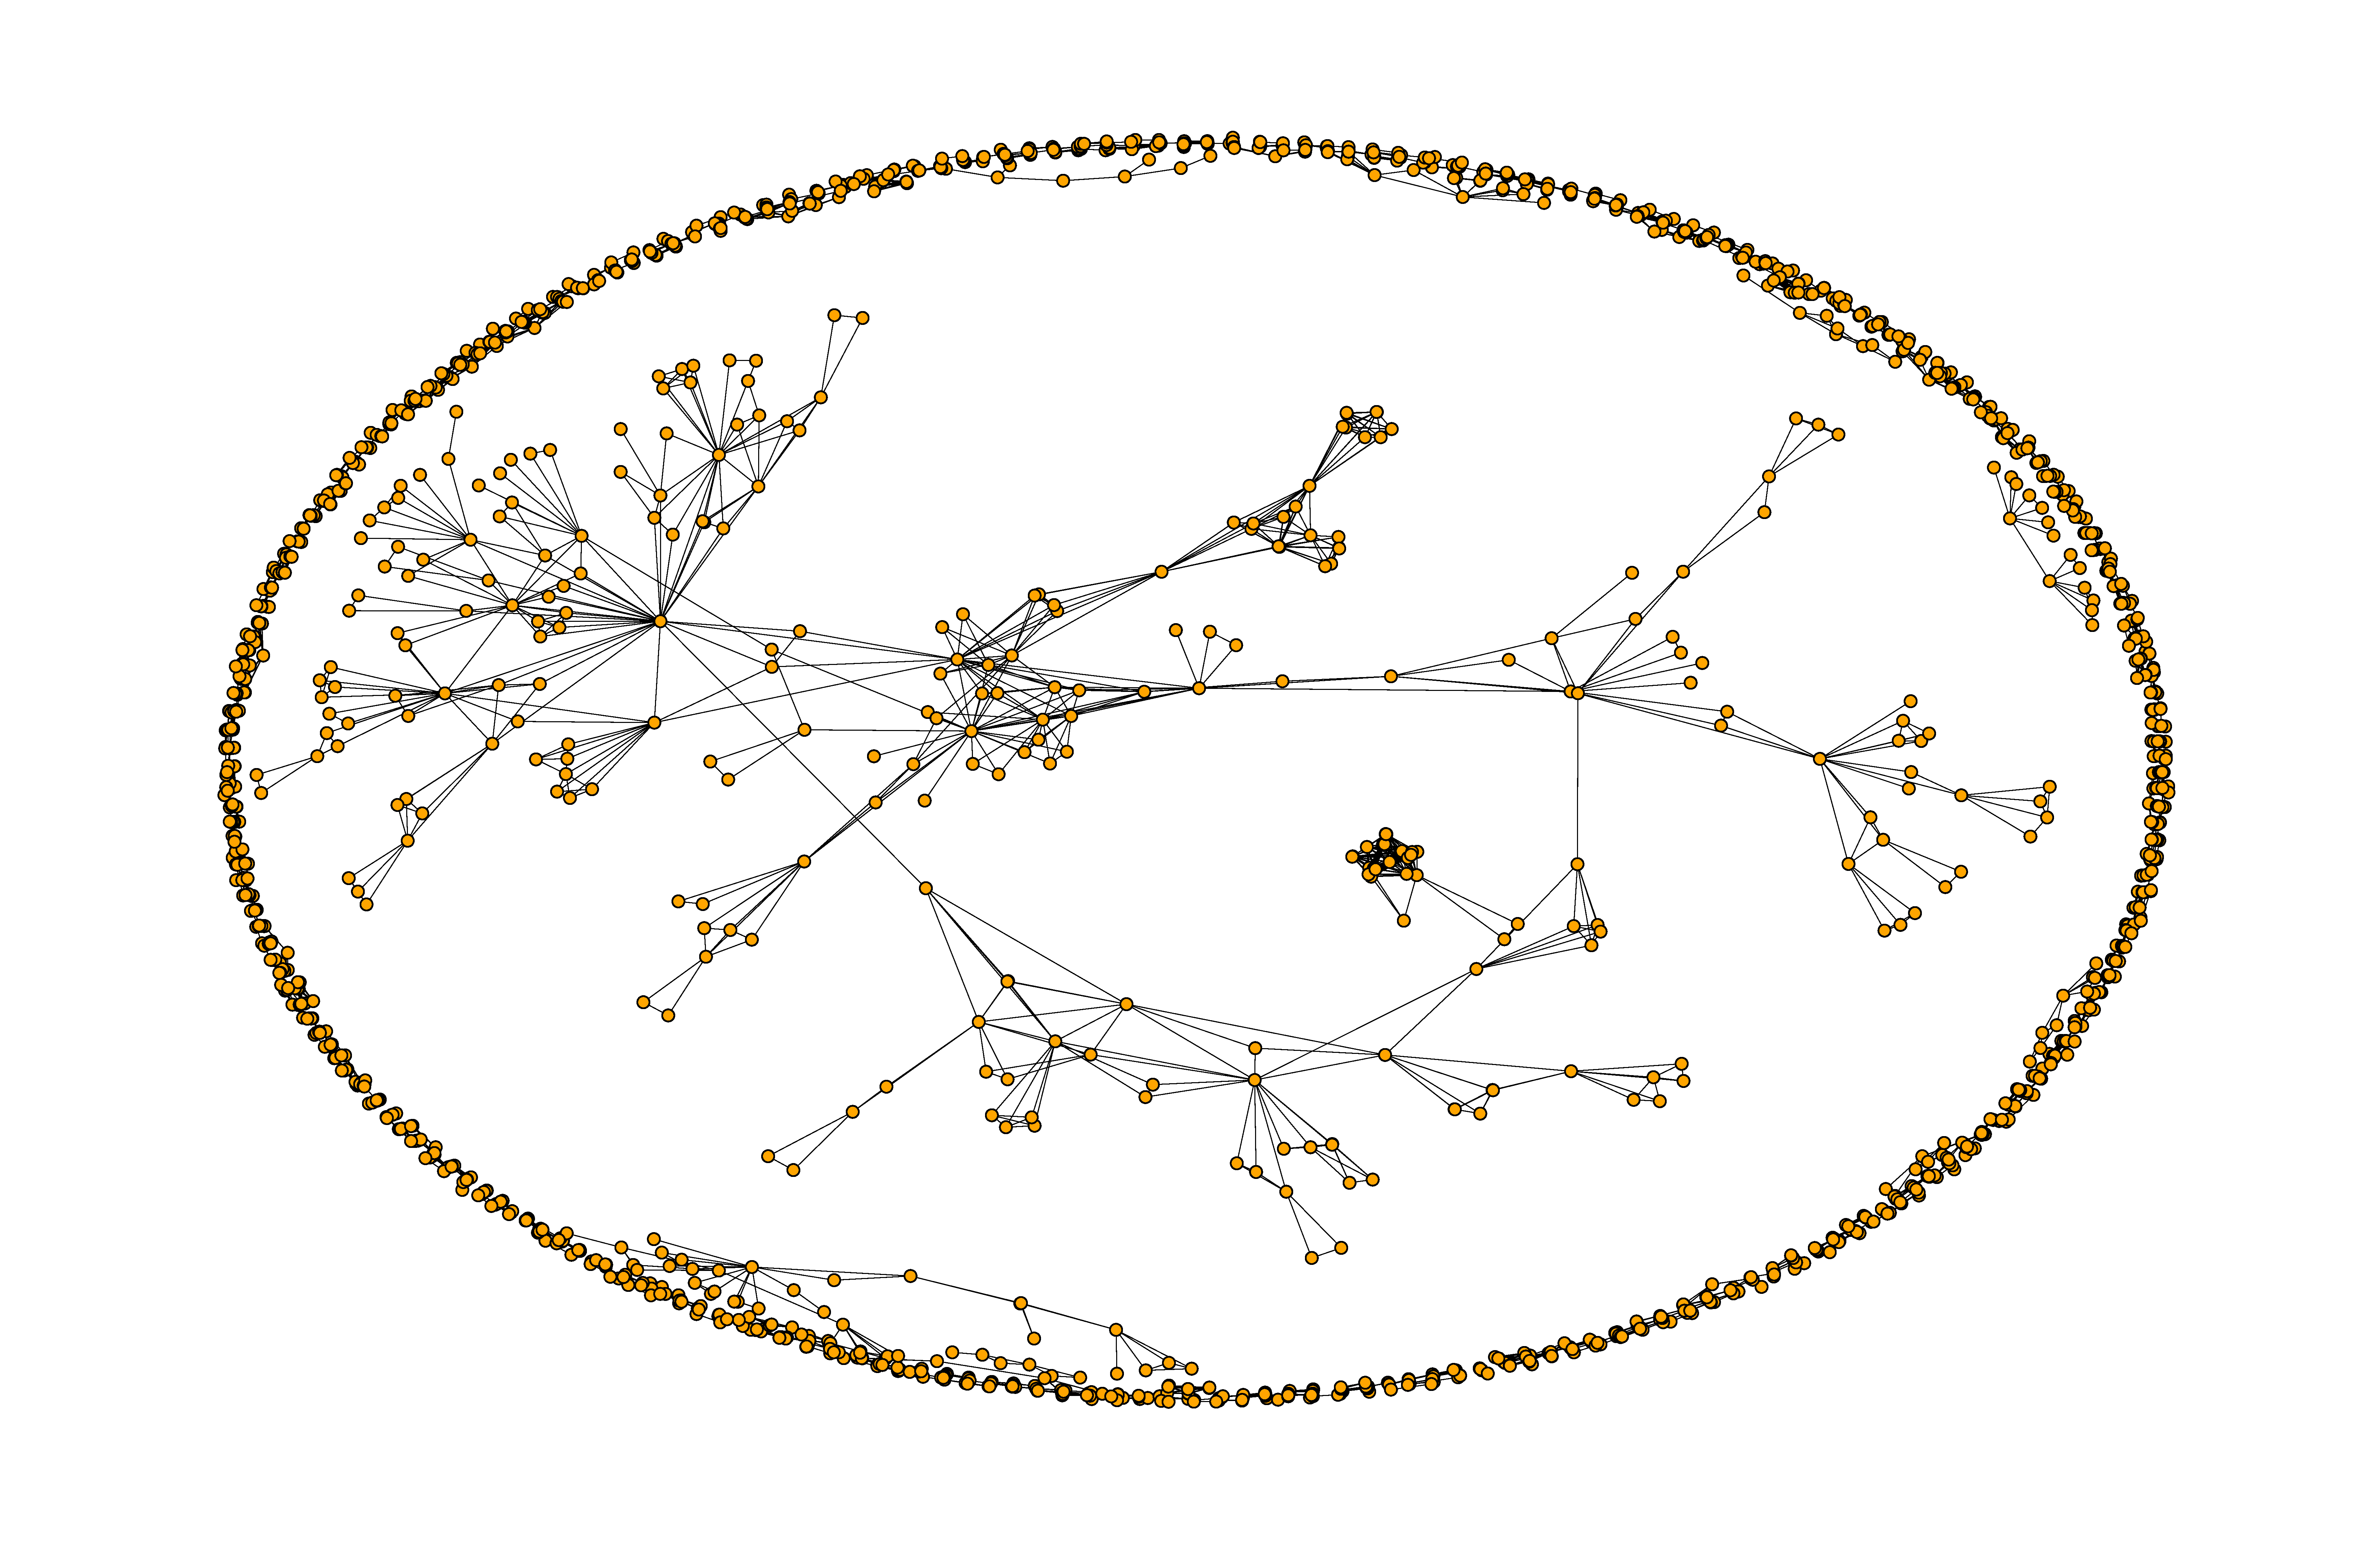
\includegraphics[width=0.6\textwidth]{./assets/images/co-authors-network.pdf}
    \caption{Co-authorship network.}\label{fig:authors_network}
\end{figure}

\begin{table}[!hbtp]
    \begin{center}
    \begin{tabular}{lr}
\toprule
{} &  unique\_key \\
author          &             \\
\midrule
martin a. nowak &          11 \\
hisao ishibuchi &          13 \\
yamir moreno    &          13 \\
zhen wang       &          13 \\
angel sánchez   &          16 \\
long wang       &          16 \\
gyorgy szabo    &          19 \\
daniel ashlock  &          21 \\
attila szolnoki &          29 \\
matjaz perc     &          34 \\
\bottomrule
\end{tabular}

    \end{center}
    \caption{Top 10 most published authors.}
    \label{table:most_published}
\end{table}

\begin{figure}[!hbtp]
    \centering
    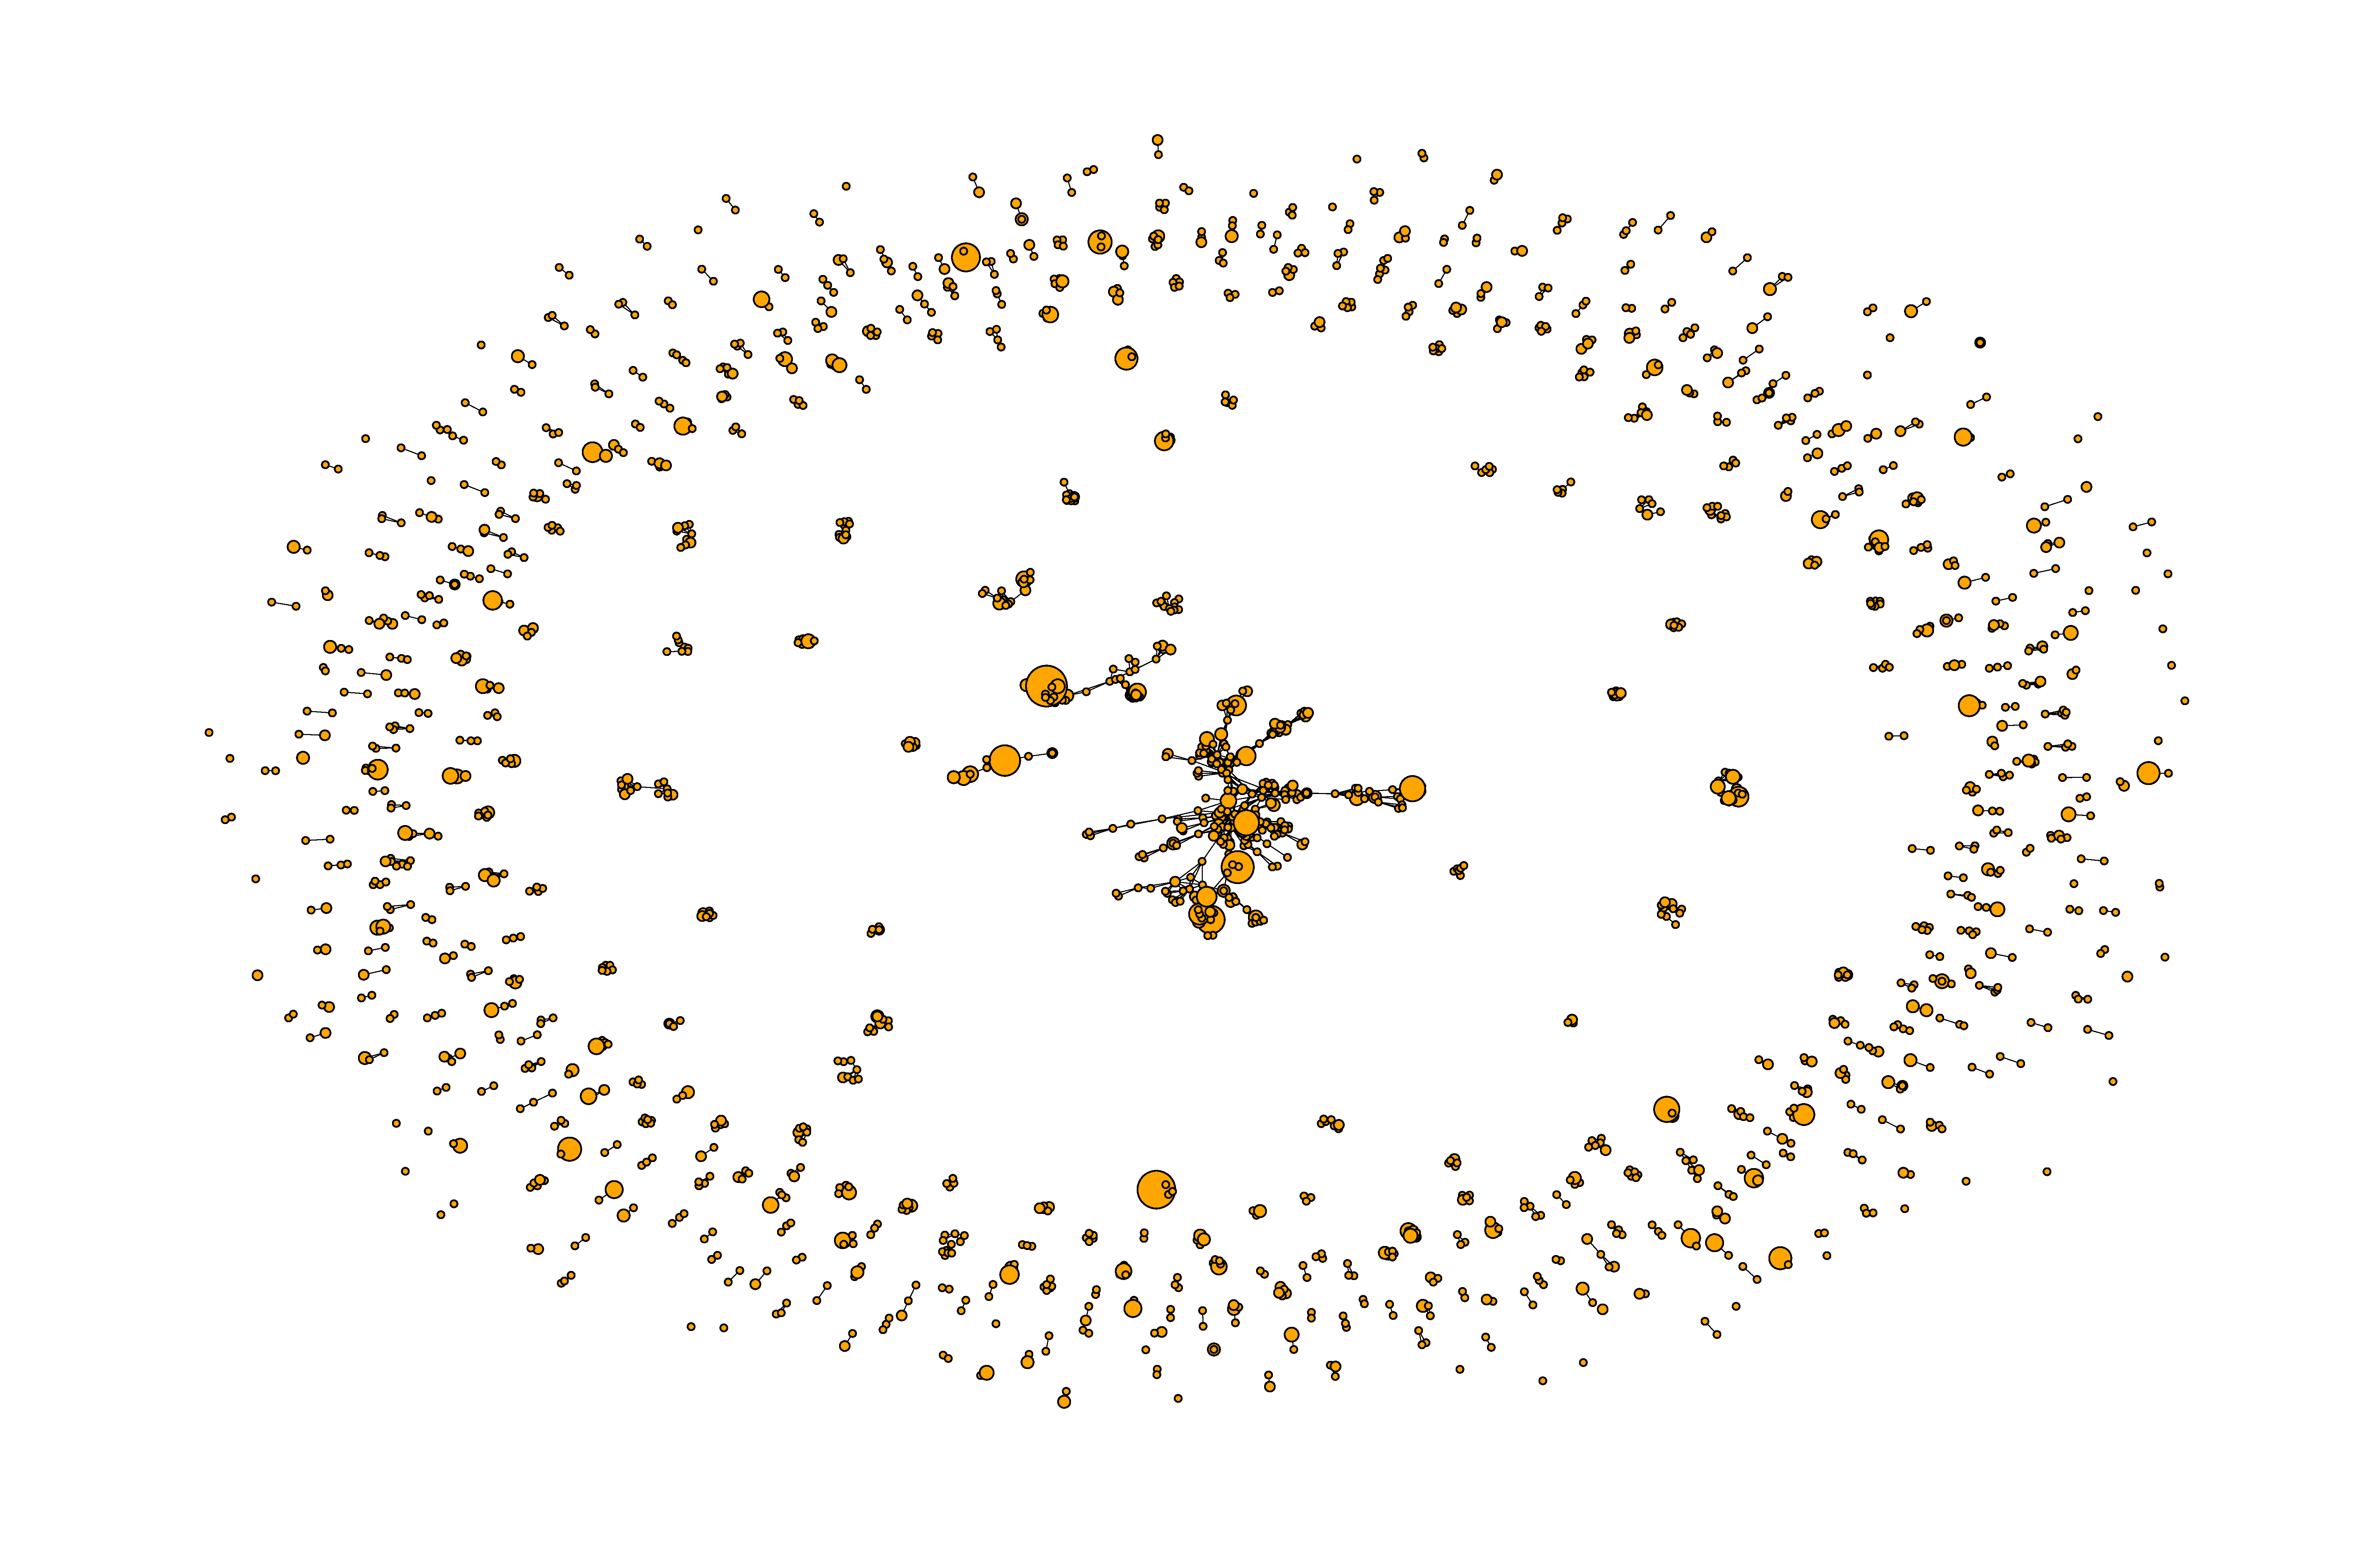
\includegraphics[width=0.6\textwidth]{./assets/images/co-authors-network-weight.pdf}
    \caption{Co-authorship network with vertices' weight.}
    \label{fig:authors_network_weighted}
\end{figure}

Furthermore, the edge weight corresponds to the number of times the authors
wrote together. From Figures~\ref{fig:authors_network}, \ref{fig:authors_network_weighted}
it can bee seen that overall the co-authors network is disjoint. Several researchers
on the outer circle seem to have written alone or have a single connection to
another researcher. On the other hand, in the inner circle of the network some
connectivity of the vertices does seem to exist, with a single large cluster
located in the middle of the network.

The authors that cover the outer space, that seem to be less collaborative,
are not authors that have single contributions to the field. On the other hand
authors that have repeatedly published on the topic are located in both the outer
and inner circles of the network.

More insights can be gained by reviewing several network measures such as the
density, the average degree and centrality measures~\cite{bakshi2009}. The first
measure to be considered is the density of the network. The density of a network
is given by, \(\frac{2E}{V(V -1)}\) and is calculated to be 0.00163. The density
is defined as the ratio of the number of edges and the number of possible edges.
Thus a small value as 0.00163 indicates that the network as a low connectivity.
Another measure closely related to the density is the average degree. The average
degree is given by \(\frac{2E}{V}\) and has been calculated to be 3.22. The
histogram of the the degree distribution is given by Figure\ref{fig:degree_hist_pd}.
The most frequent degree appears to be that of 2 degrees.

\begin{figure}
    \begin{center}
    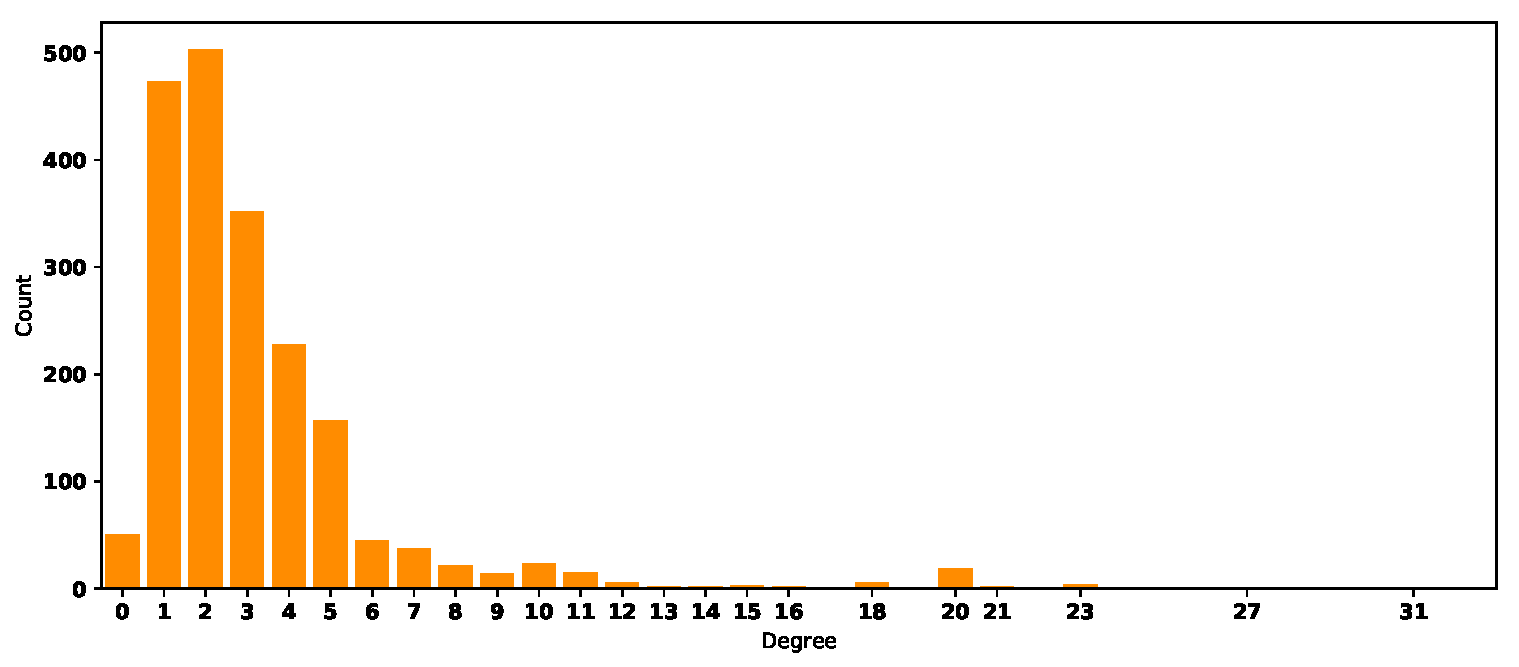
\includegraphics[width=.8\textwidth]{./assets/images/degrees_hist_pd.pdf}
    \caption{Degree Histogram. Co-authors network of prisoner's dilemma data.}
    \label{fig:degree_hist_pd}
    \end{center}
\end{figure}

Furthermore we compute node centrality measures. Indicators of centrality
identify the most important vertices of the network. There are several centrality
measures, for the purpose of this work the following are considered:

\begin{itemize}
    \item weighted betweenness centrality;
    \item closeness centrality;
    \item weighted page rank;
\end{itemize}

The results of the different centrality measures are given by Table~\ref{table:central_authors_pd}.
Though several differences between the ranks of the three measures are spotted,
some names appear to be on the most central vertices for all three measures.
These are authors:

\begin{itemize}
    % TODO Add these people to the timeline section.
    \item Matjaz Perc;
    \item Yamir Moreno;
    \item Arne Traulsen;
    \item Martin A. Nowak;
    \item Angel Snchez;
    \item Krishnendu Chatterjee.
\end{itemize}

In agreement of all measures the above are the most central authors of our network.
More specifically, the most central author is Matjaz Perc.

Though several insights were gained from studying the authorship within the field
we do not know how these findings compare to either fields. For example, an
average degree of 3.22 means that the field is more collaborative than other or not?
These questions are delved into in the following section.

\begin{table}[!hbtp]
    \begin{center}
    \scalebox{0.8}{
    \begin{tabular}{llr}
\toprule
{} &      Author name &  Betweeness \\
\midrule
1 &      Matjaz Perc &    0.010584 \\
2 &     Yamir Moreno &    0.008786 \\
3 &    Luo-Luo Jiang &    0.004319 \\
4 &    Arne Traulsen &    0.003920 \\
5 &  Martin A. Nowak &    0.003832 \\
\bottomrule
\end{tabular}

    \begin{tabular}{llr}
\toprule
{} &    Author name &  Closeness \\
\midrule
0 &    Matjaz Perc &   0.044428 \\
1 &   Yamir Moreno &   0.043561 \\
2 &   Cheng-Yi Xia &   0.038910 \\
3 &  Sandro Meloni &   0.037959 \\
4 &  Alberto Aleta &   0.037600 \\
\bottomrule
\end{tabular}

    \begin{tabular}{llr}
\toprule
\(R_3\) &      Author name &  Page rank \\
\midrule
0 &            Matjaz Perc &   0.004066 \\
1 &        Attila Szolnoki &   0.003036 \\
2 &         Daniel Ashlock &   0.002711 \\
3 &          Angel Sánchez &   0.002607 \\
4 &              Long Wang &   0.002577 \\
5 &           Yamir Moreno &   0.002260 \\
6 &              Zhen Wang &   0.002179 \\
7 &           Gyorgy Szabo &   0.002067 \\
8 &  Krishnendu Chatterjee &   0.001834 \\
9 &        Martin A. Nowak &   0.001822 \\
\bottomrule
\end{tabular}
}
    \caption{Central authors based on different centrality measures.}
    \label{table:central_authors_pd}
    \end{center}
\end{table}

\subsubsection{Comparison with other topics authorship}

In order to achieve objective insights regarding authorship in the field of the
prisoner's dilemma we perform a comparison in this section. We compare how well connected the
network of authors for the prisoner's dilemma is compared to other topics.
The data collected are on two different topics within game theory, these are:

\begin{itemize}
    \item price of anarchy and
    \item auction games.
\end{itemize}

The open source project Arcas was used again, this time using the following
keywords respectively for each topic,

\begin{itemize}
    \item key: price of anarchy;
    \item key: auction game theory.
\end{itemize}

A summary of the two data set is given by Table~\ref{table:data_sets_summary}.
A total of 296 unique articles have been collected on price of anarchy. The
earliest entry being in 2003 and a total of 668 unique authors have written about
the topic. In comparison, a total of 2103 articles are examined for auction
games. Auction games are a well studied topic for several years with the earliest entry
going back to 1974. Finally, 3860 different names are examined. The frequency
of the prisoner's dilemma, for both articles and authors, lies between the frequencies
of these two topics. In Figure~\ref{fig:timeplots_anarchy_auction} a timeplot for each
topic is displayed and is exhibited that both topics have an increasing trend over
the years. Though price of anarchy is clearly a new topic compared to auction games.

\begin{table}[!hbtp]
    \begin{center}
    \begin{tabular}{llr}
        \toprule
         &            Price of anarchy &  Auction games \\
        \midrule
        Unique articles      & 296  & 2103 \\
        Unique authors       & 668  & 3860 \\
        Min publication year & 2003 & 1974 \\
        Max publication year & 2017 & 2017 \\
        \bottomrule
    \end{tabular}
    \end{center}
    \caption{Data sets summary.}\label{table:data_sets_summary}
\end{table}

\begin{center}
\begin{figure}[!hbtp]
    \begin{subfigure}{0.5\textwidth}
        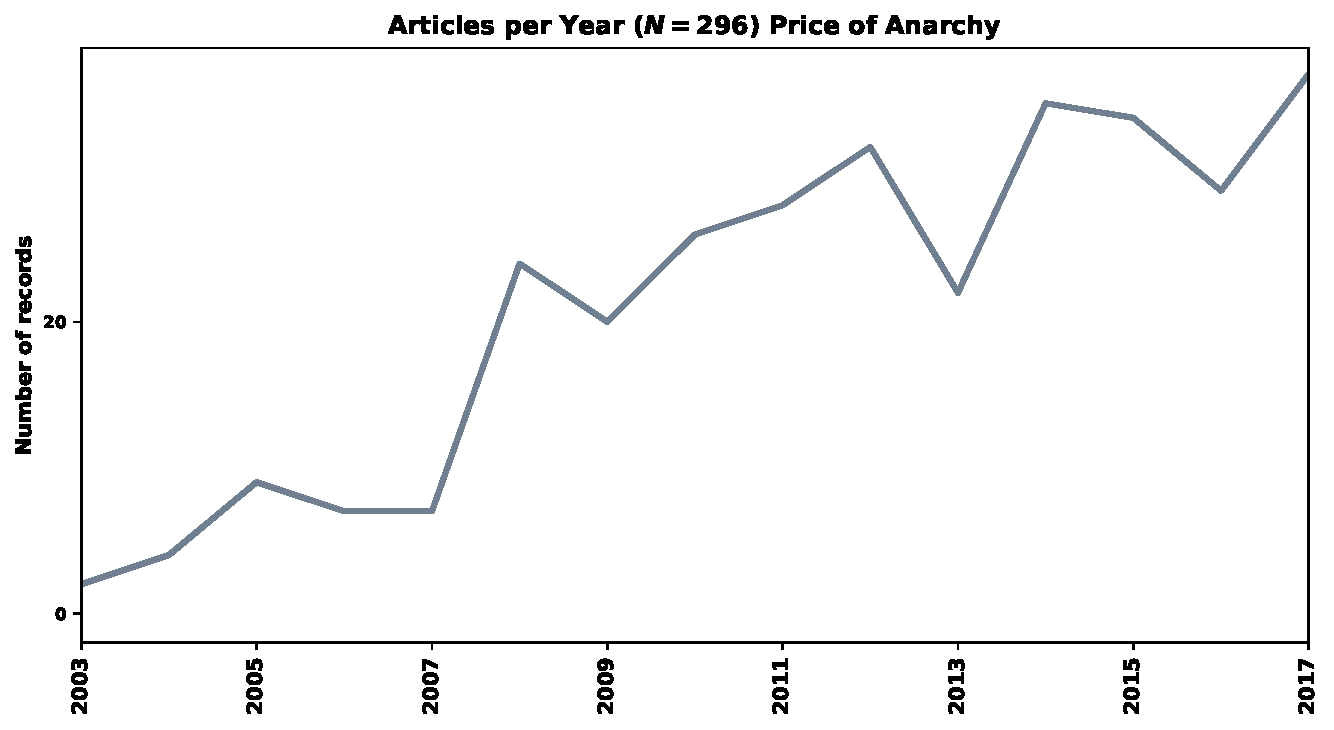
\includegraphics[width=\textwidth]{./assets/images/anarchy_timeline.pdf}
    \end{subfigure}
    \begin{subfigure}{0.5\textwidth}
        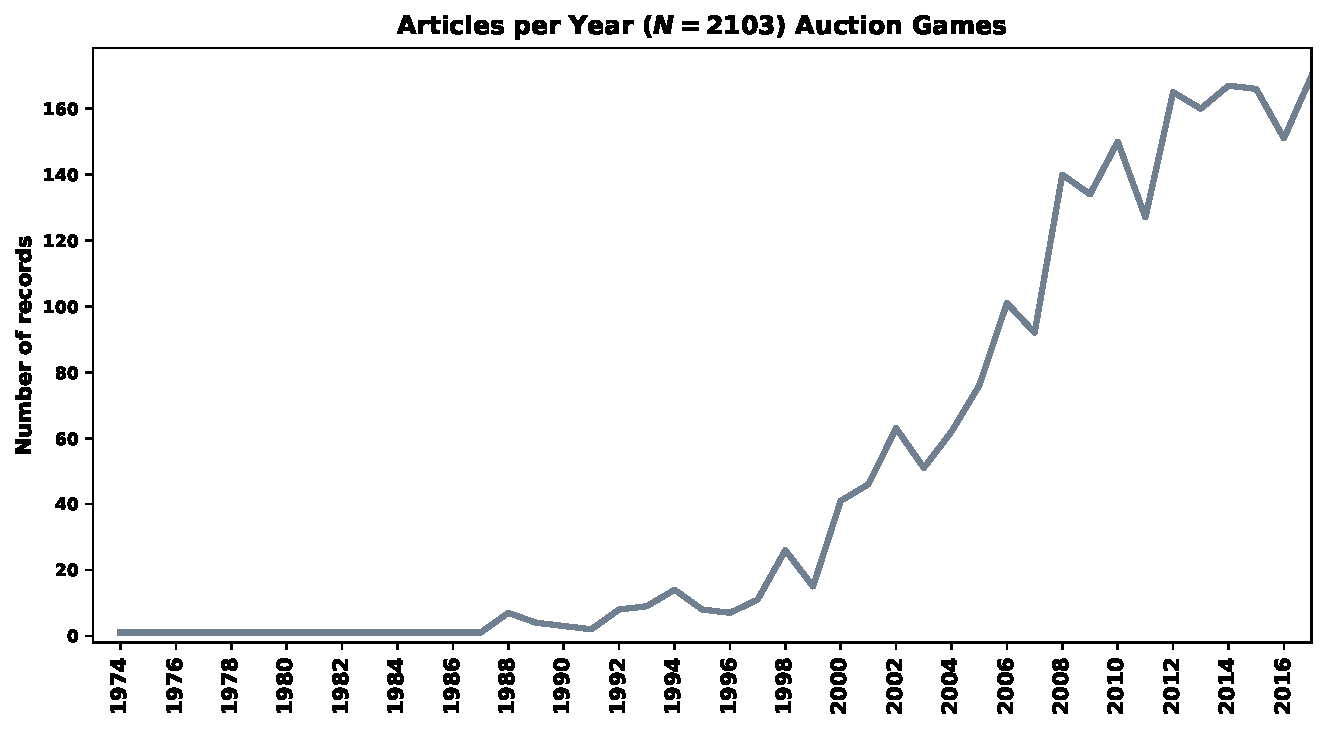
\includegraphics[width=\textwidth]{./assets/images/auction_timeline.pdf}
    \end{subfigure}
\caption{Timeplots.}\label{fig:timeplots_anarchy_auction}
\end{figure}
\end{center}


The immediate step is to compare the networks we have constructed for all three
fields. The aim of the comparison is to gain insight as to how collaborative
the prisoner's dilemma authors are compared to other fields. Network measures
discussed in this comparison are given by Table~\ref{table:descriptive_networks}.
The smallest network is that of the authorship describing the price of anarchy,
followed by the prisoner's dilemma and the largest one is that of the auction
games. The average degree (calculated as \(\frac{2E}{V}\)), is for all three
networks is close to 3 and the density of all networks is very small, less than
0.005.

\begin{table}[!hbtp]
    \begin{center}
    \begin{tabular}{cccc}
\toprule
& Prisoner's Dilemma & Price of anarchy &  Auction games \\
\midrule
\(\mid V \mid \)                   & 1970    & 637 & 3968 \\
\(\mid E \mid \)                   & 3179    & 865 & 5713 \\
Density                            & 0.00163 & 0.00427 & 0.00072\\
Average degree                     & 3.22    & 2.71 & 2.87 \\
\bottomrule
    \end{tabular}
    \end{center}
    \caption{Descriptive measures of networks.}\label{table:descriptive_networks}
\end{table}

To further examined the differences or the similarities of these networks we
consider the degree distributions. The normalised distributions of all
three networks are given in Figure~\ref{fig:degrees_dist}. They have been normalised
such that the frequencies sum to one. The distributions appear to be similar
but to validate the hypothesis a statistical test will be used. None of the
distributions is normally distributed thus the non parametric test Kruskal-Wallis
is used~\cite{mckight2010}. Kruskal-Wallis allow us to compare the medians of
two or more distributions. The test returns a \(p\)-value of 0.29. Thus, there is no
significant difference in the degree distributions of the three networks.

\begin{figure}[!hbtp]
    \centering
    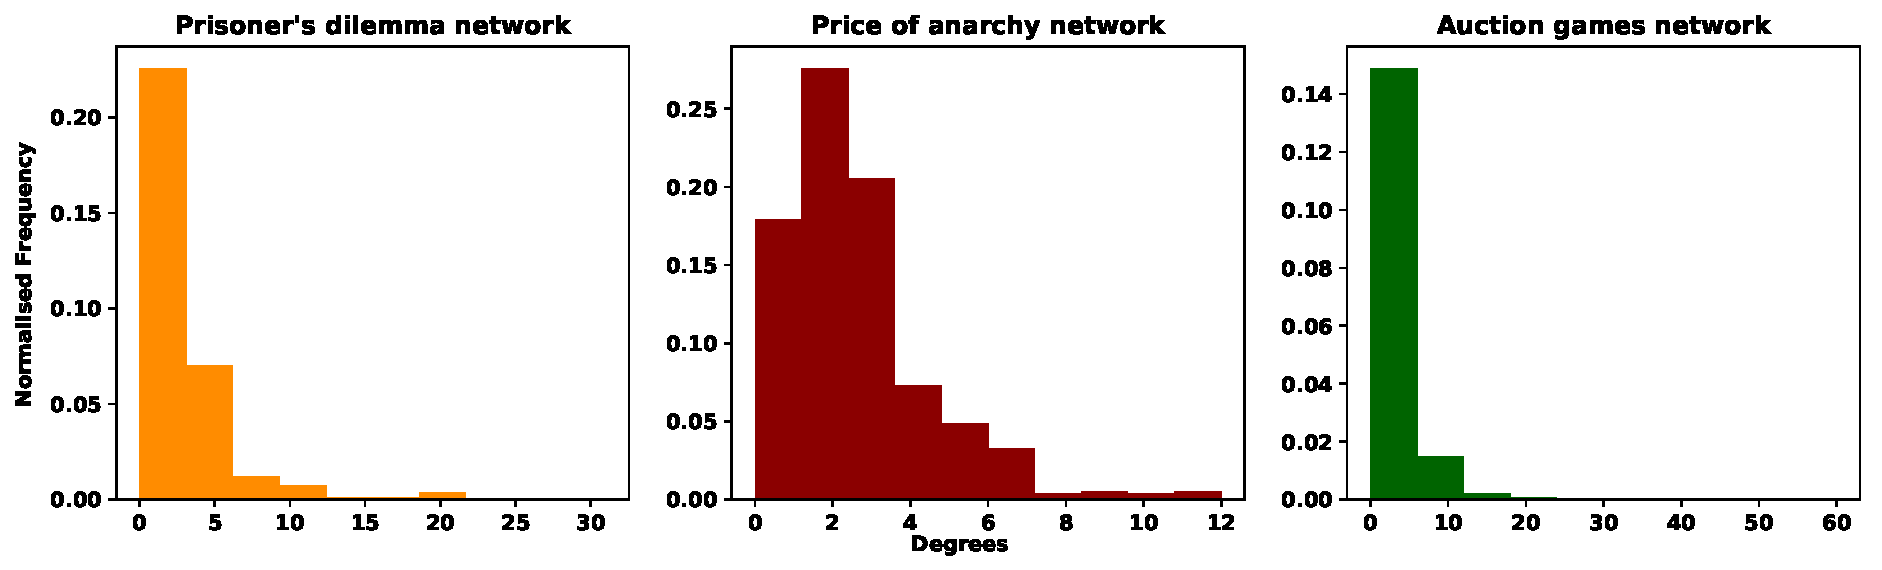
\includegraphics[width=\textwidth]{./assets/images/degrees_histrograms.pdf}
    \caption{Degree distributions for all three networks.}\label{fig:degrees_dist}
\end{figure}

An interesting insight can be gained by examining the evolution of both the
average and the median degree over time. Though when the entire data sets are
considered the average degree of all networks is close to 3, when observing
the previous year this does not seem to be the case. The evolution of the
degrees over the publication years of each topic have been very different.
This can be observed by Figures~\ref{fig:av_degrees_over_time} and
\ref{fig:md_degrees_over_time}. Auction games have had an increasing trend in
co-authorships over time. The prisoner's dilemma study, though it does have an
increasing trend has two sudden jumps. A decrease occurred in 1960 and a sudden
increase in 1970. Finally, the price of anarchy had a big increase in authorship
in 2004.

\begin{figure}[!hbtp]
    \centering
    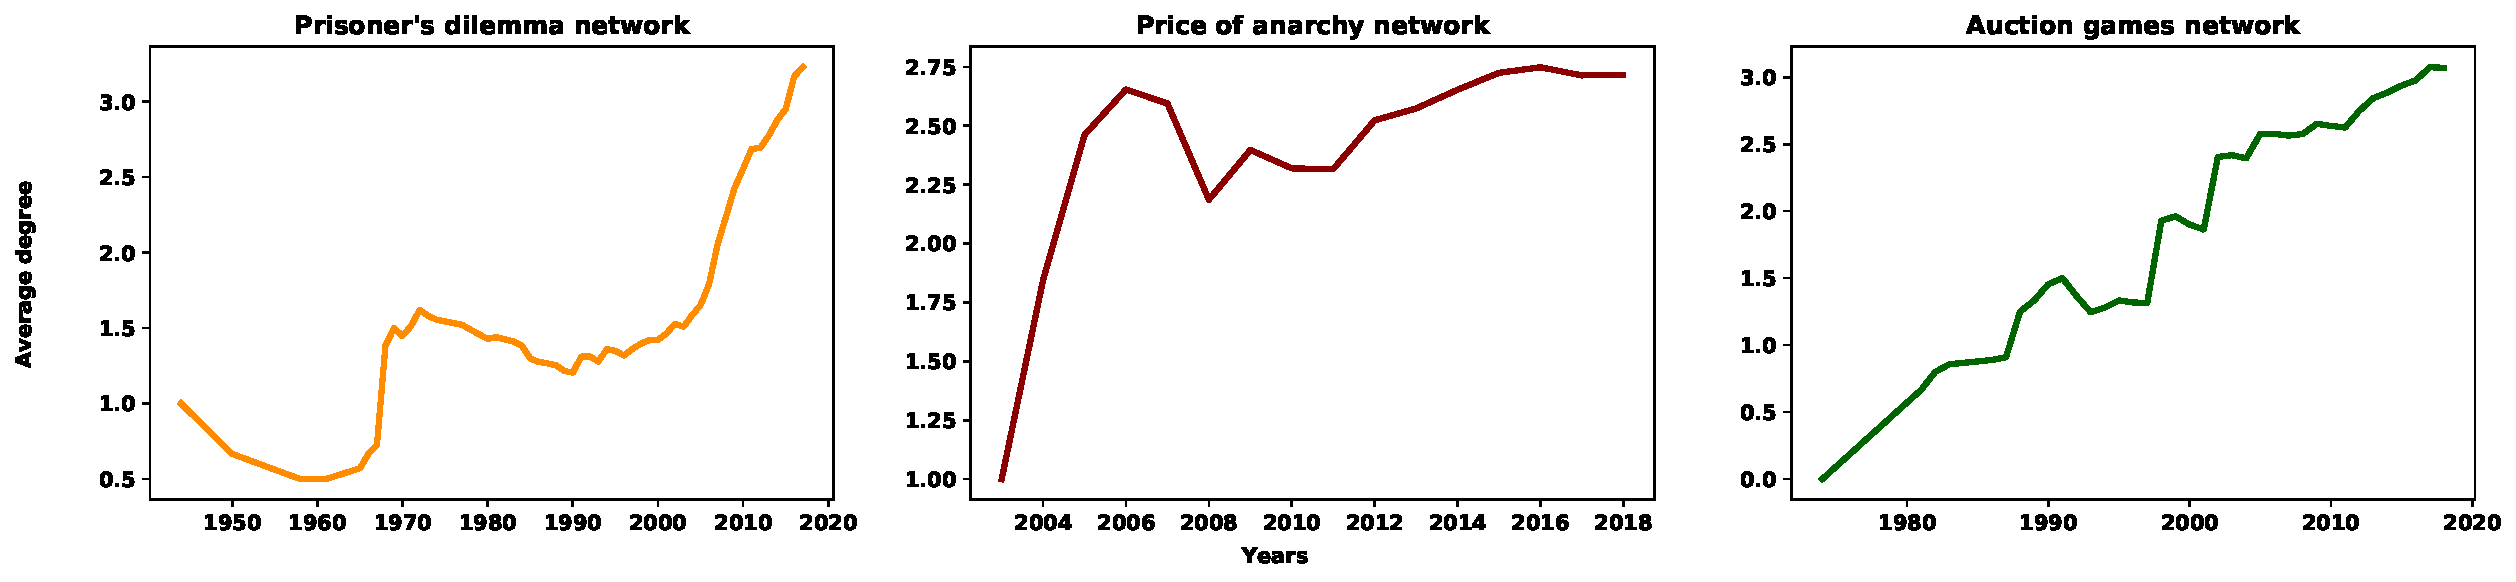
\includegraphics[width=\textwidth]{./assets/images/average_degrees_lineplots.pdf}
    \caption{Average degree over time for all three networks.}
    \label{fig:av_degrees_over_time}
\end{figure}

\begin{figure}[!hbtp]
    \centering
    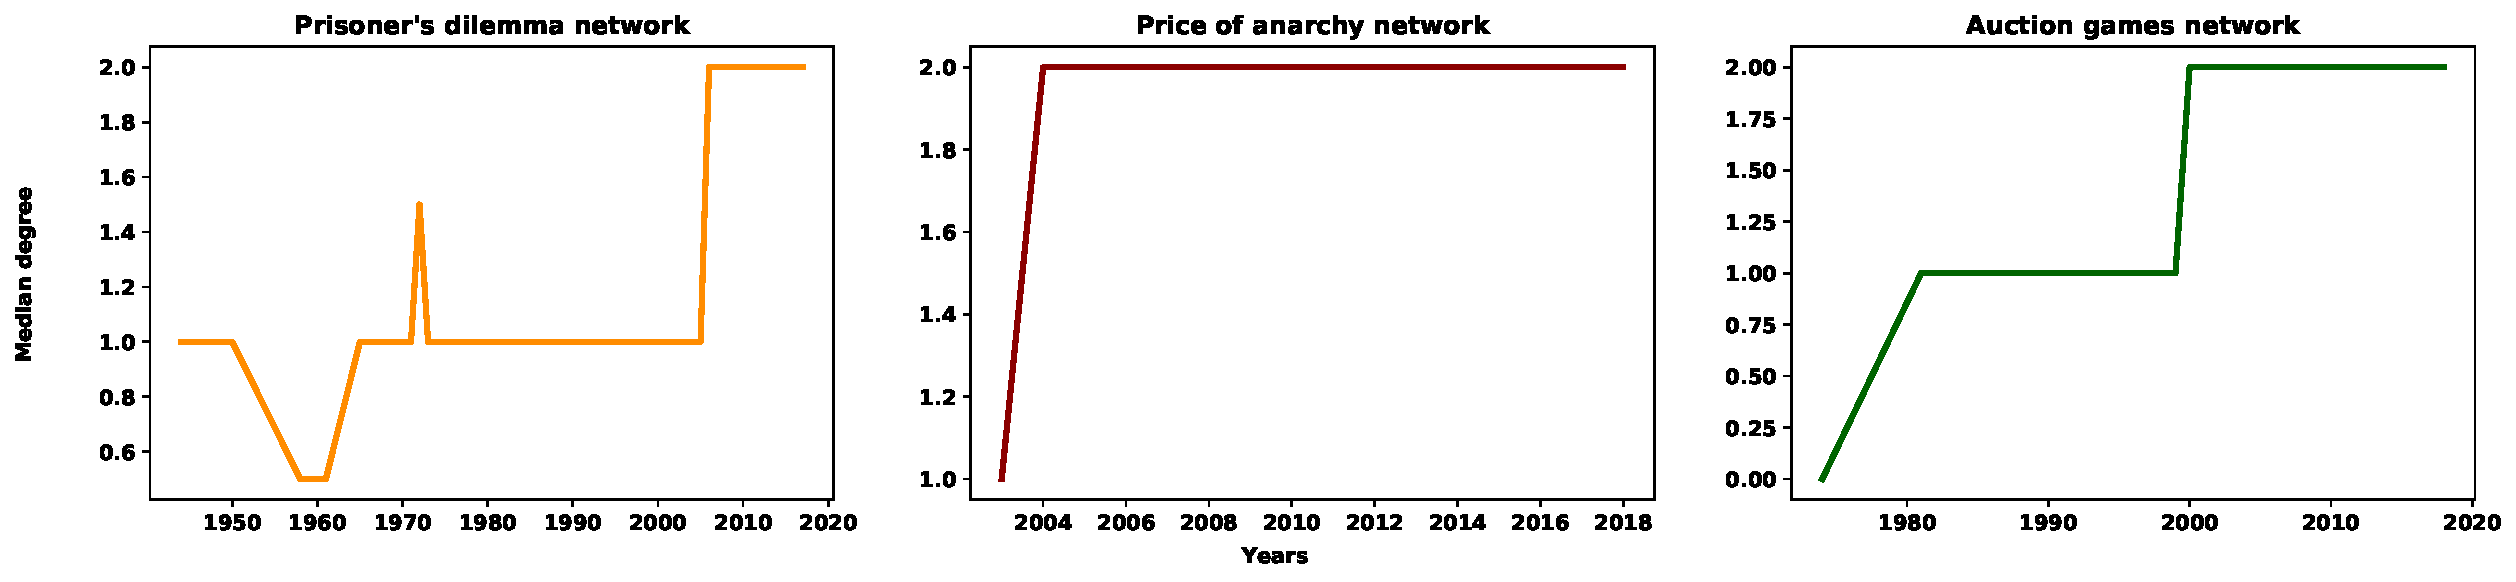
\includegraphics[width=\textwidth]{./assets/images/median_degrees_lineplots.pdf}
    \caption{Median degree over time for all three networks.}
    \label{fig:md_degrees_over_time}
\end{figure}

Other measures that could highlight similarities in the connectivity of the graphs
are centrality measures. A summary of the maximum, mean and median centrality
value based on three centrality measures for all three networks is given by
Table~\ref{table:summary_centrality_networks}. The individual histograms
are illustrated in Figures~\ref{fig:w_betweenness_hist},~\ref{fig:closeness_hist}
and~\ref{fig:page_rank_hist}. A normality test has been performed for each of the
9 distributions and with a significance level of 0.05 none of the distributions
is normally distributed. Thus, a Krustal-Wallis test will be performed to test
the mean difference between the topics for each centrality measure.

\begin{table}[!hbtp]
    \begin{center}
    \begin{tabular}{lccc}
\toprule
& Prisoner's Dilemma & Price of anarchy &  Auction games \\
\midrule
Max weighted betweenness     & 0.0093     & 0.0024     & 0.0011 \\
Mean weighted betweenness    & 4.537e-05  & 0.0        &  0.0 \\
Median weighted betweenness  & 0.0        & 3.4677e-05 & 4.5096e-06 \\
Max closeness                & 0.0443     & 0.0333     & 0.0209 \\
Mean closeness               & 0.0051     & 0.0047     & 0.0007 \\
Median closeness             & 0.0015     & 0.0063     & 0.0017 \\
Max weighted page rank       & 0.0040     & 0.0063     & 0.0012 \\
Mean weighted page rank      & 0.0005     & 0.0015     & 0.0002 \\
Median weighted page rank    & 0.0005     & 0.0015     & 0.0002 \\
\bottomrule
    \end{tabular}
    \end{center}
    \caption{Summary of centrality measures.}\label{table:summary_centrality_networks}
\end{table}

\begin{figure}[!hbtp]
    \centering
    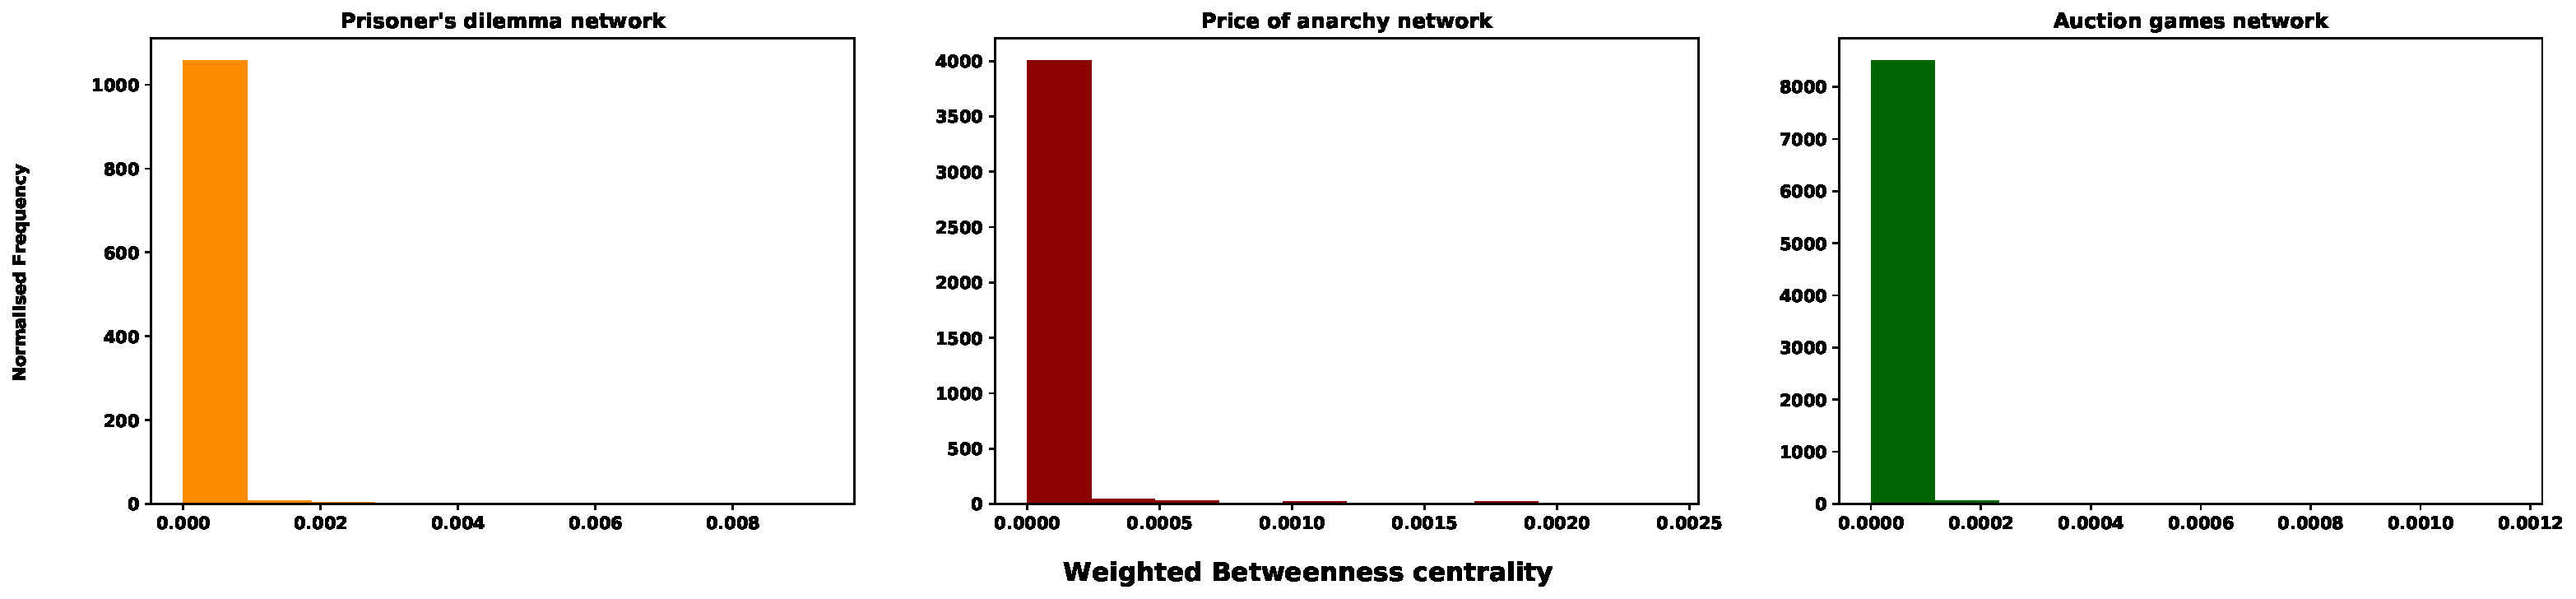
\includegraphics[width=\textwidth]{./assets/images/w_betweenness_hist.pdf}
    \caption{Between centrality histogram for all three networks.}
    \label{fig:w_betweenness_hist}
\end{figure}

\begin{figure}[!hbtp]
    \centering
    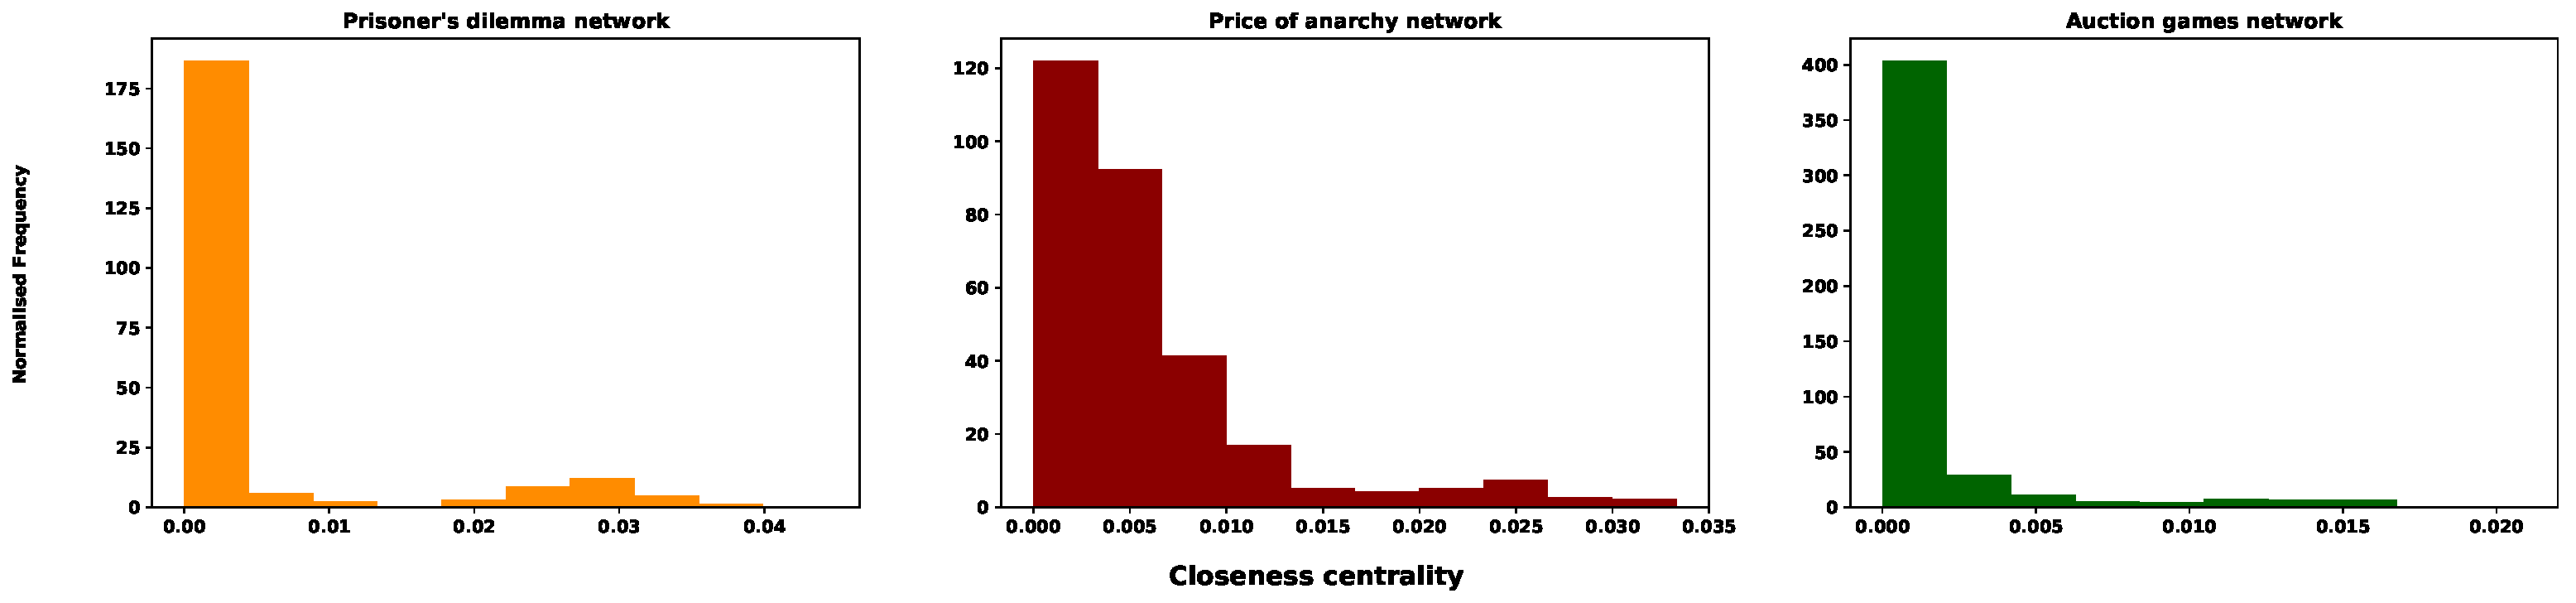
\includegraphics[width=\textwidth]{./assets/images/closeness_hist.pdf}
    \caption{Closeness centrality histogram for all three networks.}
    \label{fig:closeness_hist}
\end{figure}

\begin{figure}[!hbtp]
    \centering
    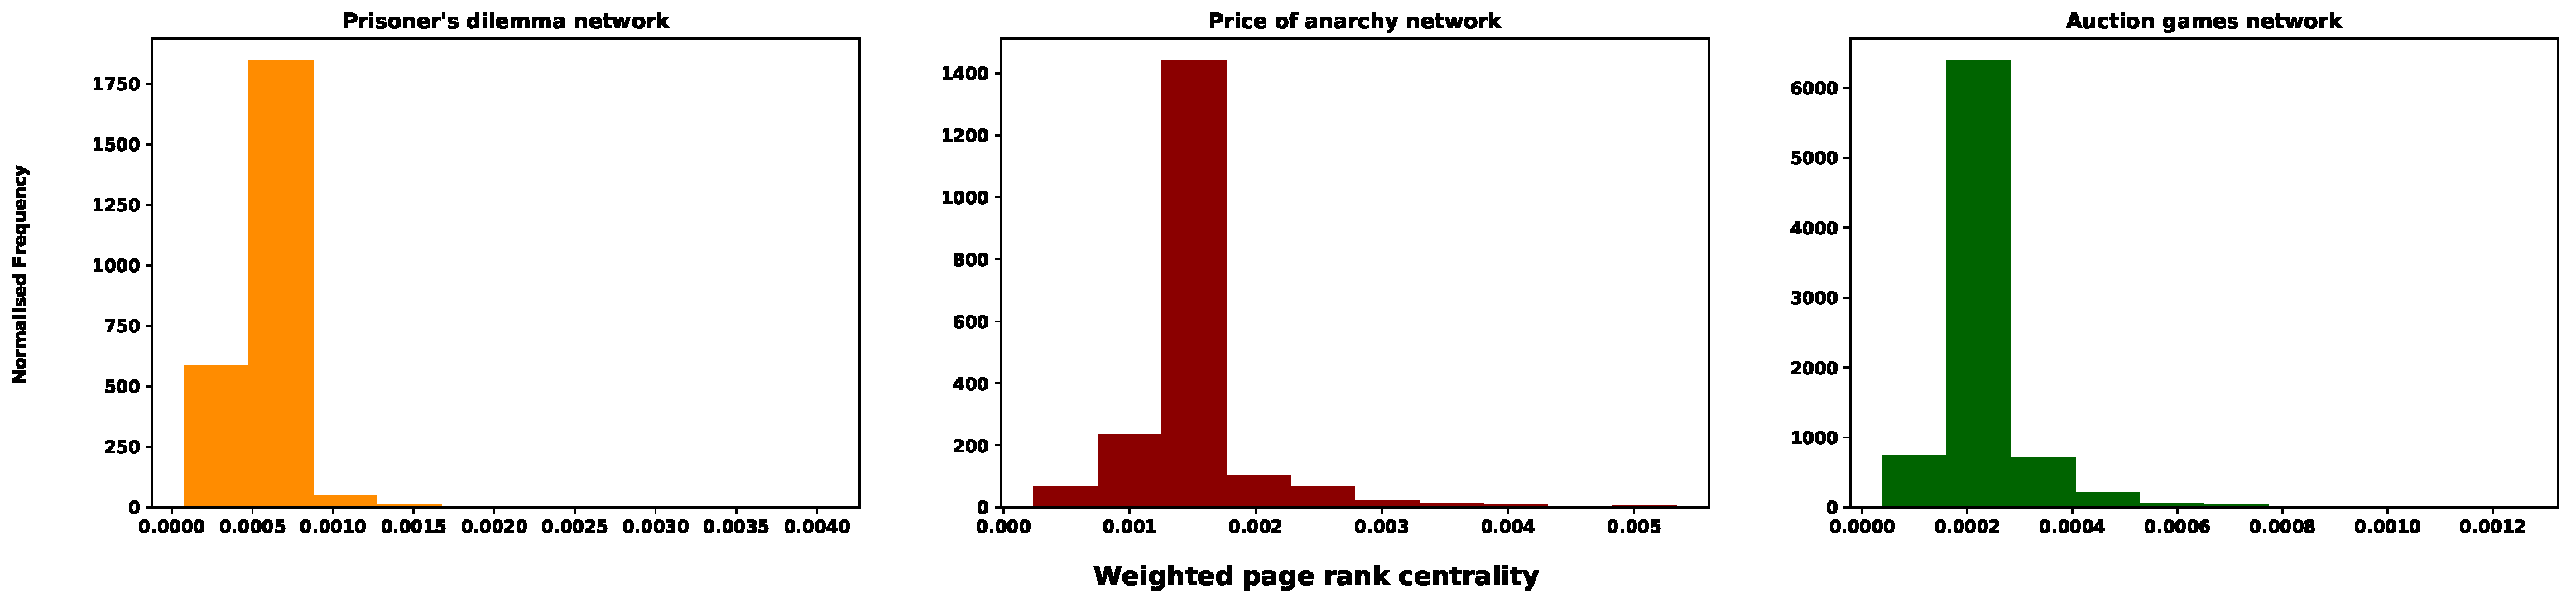
\includegraphics[width=\textwidth]{./assets/images/page_rank_hist.pdf}
    \caption{Page rank centrality histogram for all three networks.}
    \label{fig:page_rank_hist}
\end{figure}

The results of the Kruskal-Wallis tests are shown in Table~\ref{table:kruskal_wallis_results}.
It can be seen that for the closeness centrality the null hypothesis holds. Thus
there is not a significant difference of the medians. On the other hand, for
both the weighted betweenness and weighted page rank the null hypothesis is being
rejected. Thus there seems to exist a significant difference of the medians for these two
measures. A post-hoc test could be carried to further explore which medians
are significantly different.

\begin{table}[!hbtp]
    \begin{center}
    \begin{tabular}{llc}
\toprule
& \(p-\)value &   \\
\midrule
Weighted betweenness    & 0.0   \\
Closeness               & 0.799 \\
Weighted page rank      & 0.0   \\
\bottomrule
    \end{tabular}
    \end{center}
    \caption{Kruskal-Wallis tests results.}\label{table:kruskal_wallis_results}
\end{table}

In this section the amount of collaboration within the field was examined.
Furthermore, to be objective this was compared to other topics within game
theory. In the section to follow we focus on the exploration of the co-authorships
within the field of the prisoner's dilemma. The collaboration of some well known
authors alongside authors that appear to be central in our network are explored.

\subsubsection{Sub graphs analysis}
% TODO Think about what to do with this: where does it fit with the rest of the
% restructure?

In this section we explore and gain insights as to who well known authors within
our field tend to collaborate and write with. This is achieved by studying the
cliques of the network. Cliques are subsets of vertices, all adjacent to each other.
A total of 779 cliques exists within the network and the max node number of a
clique is 21. The clique with the 21 authors is from~\cite{Knight2016}.
Though a big number of cliques exists in this section we will only examine those
of authors that have been discussed several times within this work.

The first clique is that of R. Axelrod. The subgraph, shown in Figure
\ref{fig:axelrods_clique}, consists of 4 vertices, 3 edges and the edge weights
are all equal to 1. Thus for this subgraph we examined the betweenness, closeness
and page rank centrality (all without weights). The central node is Axelrod
based on all centrality measures. The results are shown in Table~\ref{table:axelrods_clique}.

Furthermore, the density of the subgraph is equal to 0.5 and the average degree
in 1.5. All authors are connected to Axelrod with a step of one. That is because
all these authors have written only with Axelrod in~\cite{Axelrod1988,
Axelrod1984, Wu1995}.

\begin{figure}[!hbtp]
    \centering
    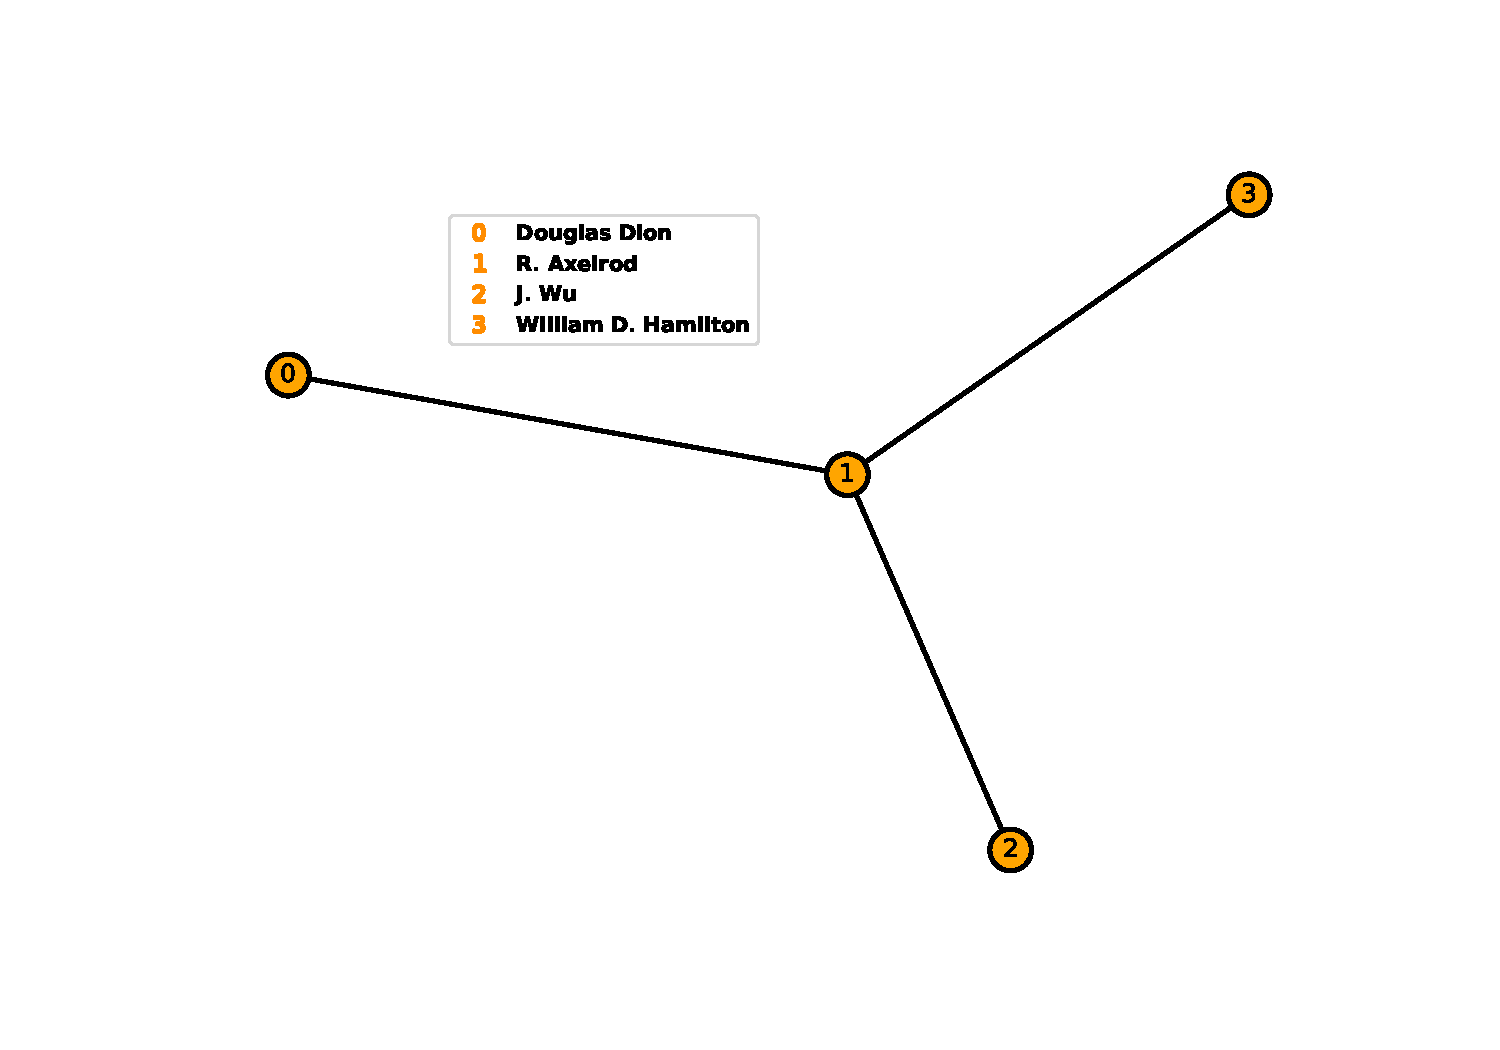
\includegraphics[width=0.6\textwidth]{./assets/images/Axelrod.pdf}
    \caption{R. Axelrod's clique.}
    \label{fig:axelrods_clique}
\end{figure}

\begin{table}[!hbtp]
    \begin{center}
    \begin{tabular}{llll}
    \toprule
    Author name &  Betweenness & Closeness & Page rank \\
    \midrule
     R. Axelrod          &    1.00 & 0.6 & 0.1734 \\
     J. WU               &    0.00 & 1.0 & 0.4797 \\
     William D. Hamilton &    0.00 & 0.6 & 0.1734 \\
     D. Douglas          &    0.00 & 0.6 & 0.1734 \\
    \bottomrule
    \end{tabular}
    \caption{Centrality measures for Axelrod's clique.}
    \label{table:axelrods_clique}
    \end{center}
\end{table}

The next clique considered is that of D. Ashlock. The subgraph which contains
Ashlock is larger than Axelrod's one. It has a total of 24 vertices
and 38 edges. The density is equal to 0.137 and the average degree is 3.16.
Moreover, based on all three centrality measures Ashlock appears to be the most
central node of this subgraph. Table~\ref{table:ashlock_clique} present the 10
most central authors.

An interesting insight can be gained by observing the length of the shortest
paths for any author to reach Ashlock. The maximum shortest path is 4. Thus,
anyone can reach Ashlock at most with 4 steps.

\begin{figure}[!hbtp]
    \centering
    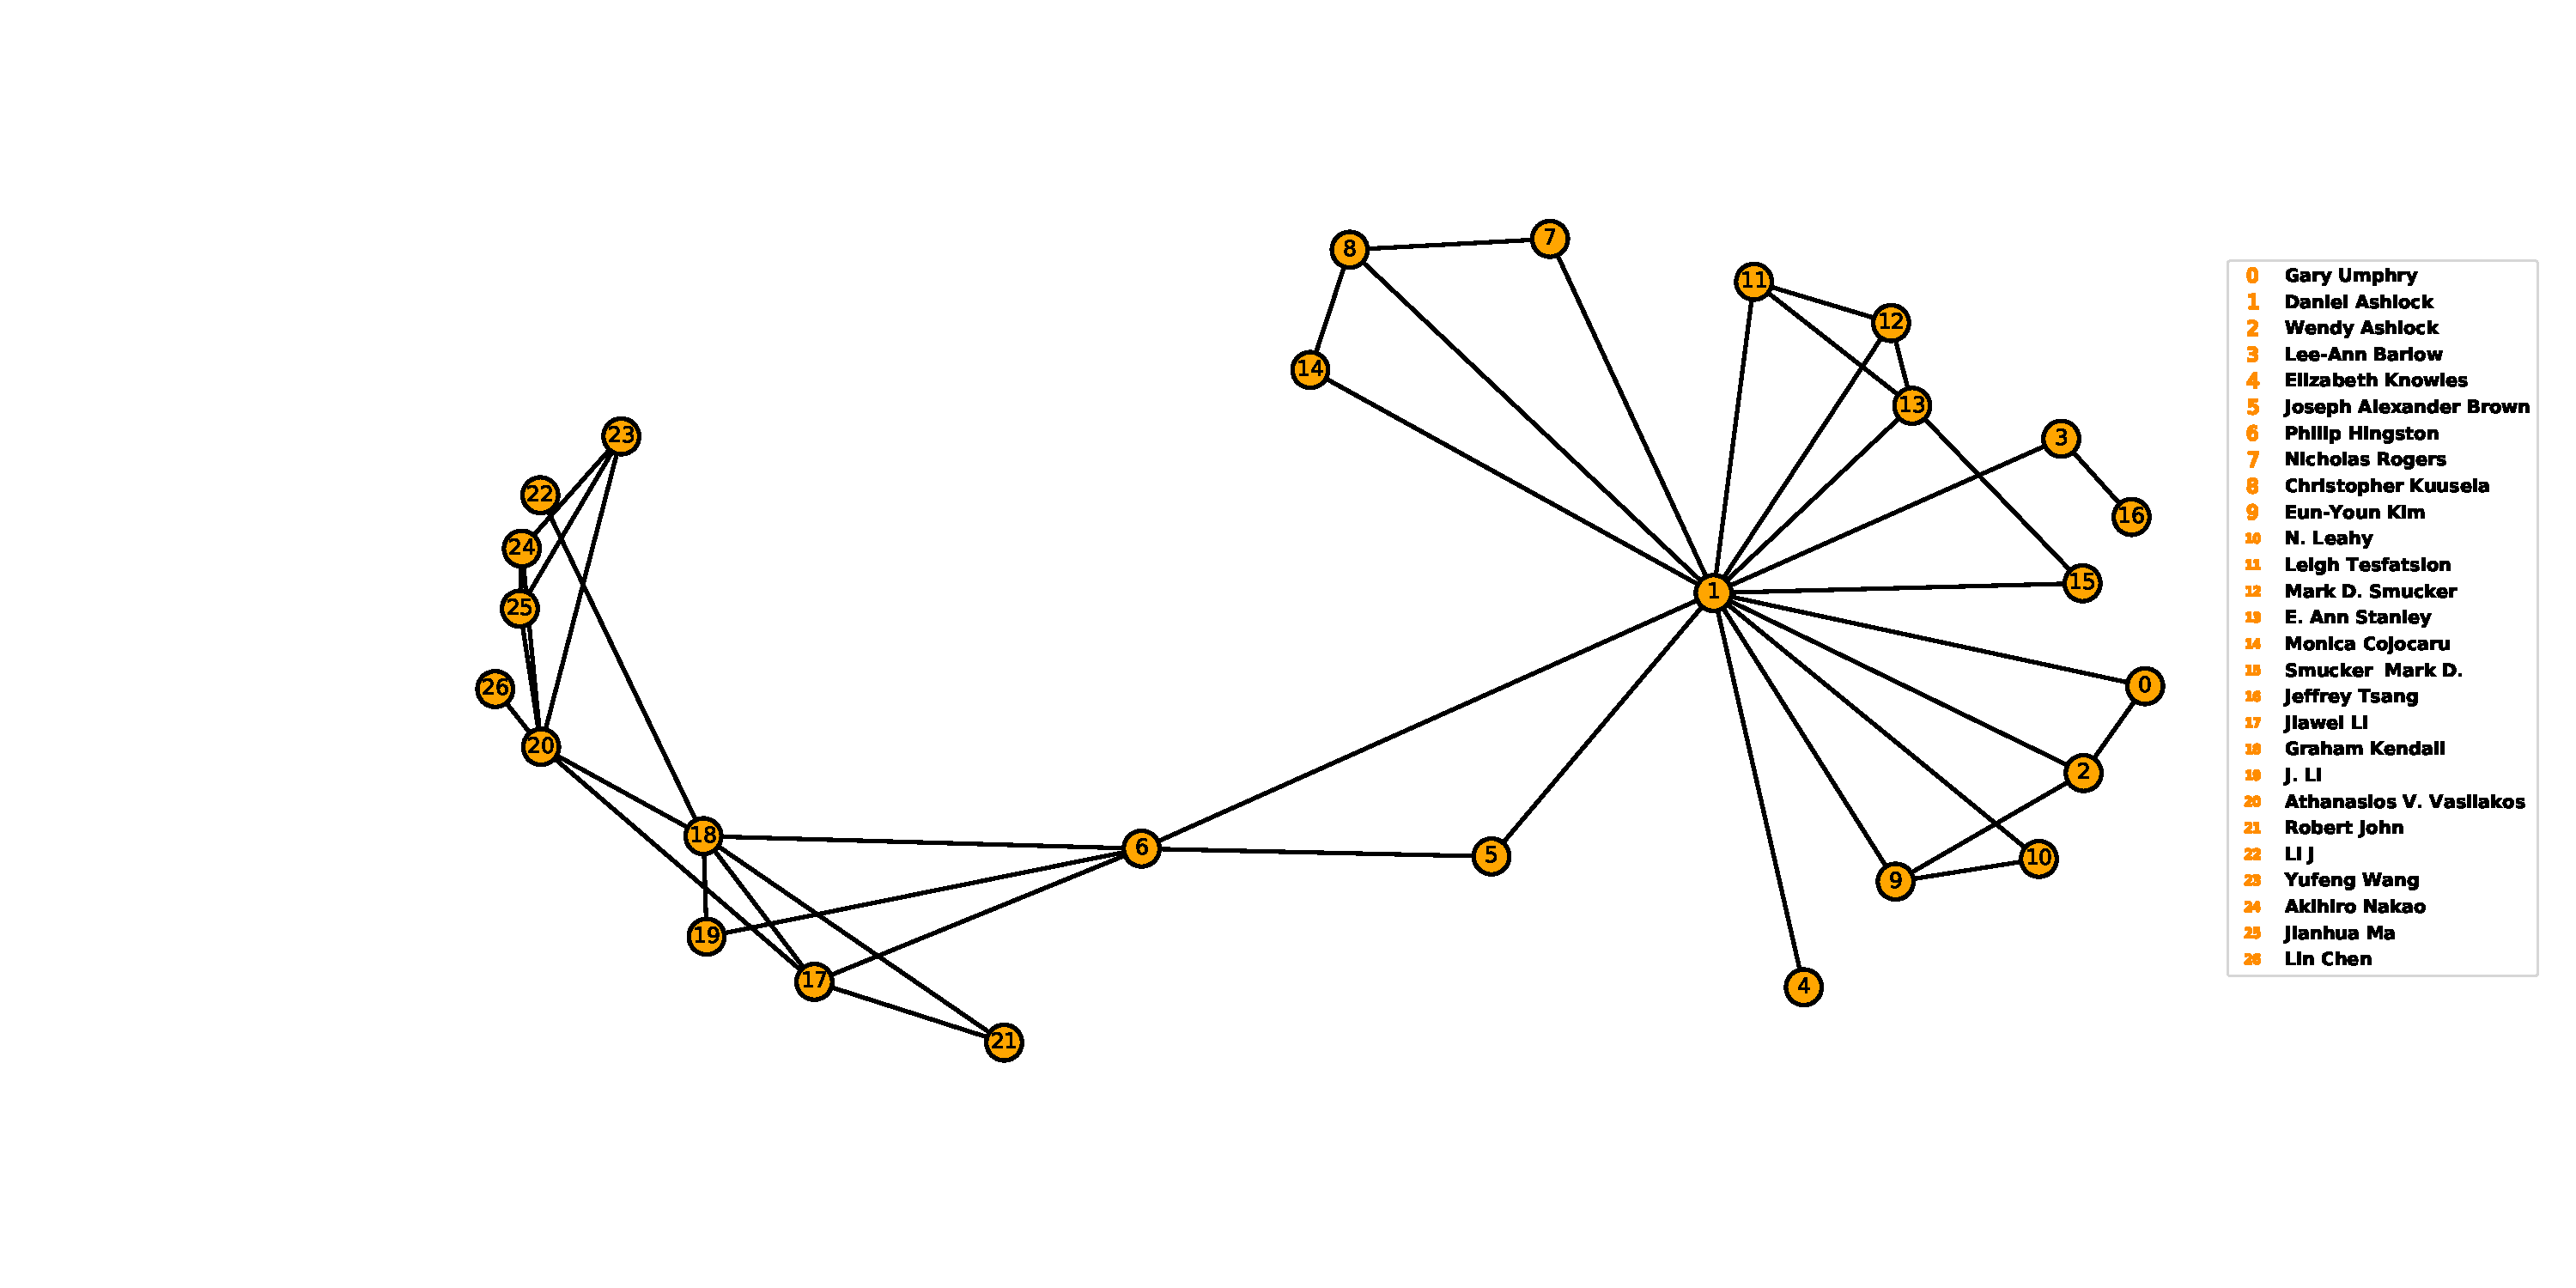
\includegraphics[width=\textwidth]{./assets/images/Ashlock.pdf}
    \caption{Subgraph that contains D. Ashlock.}
    \label{fig:ashlocks_clique}
\end{figure}

\begin{table}[!hbtp]
    \begin{center}
    \scalebox{0.8}{
    \begin{tabular}{llr}
\toprule
\(R_1\) &              Author name &  Betweenness \\
\midrule
0 &           Daniel Ashlock &                0.7806 \\
1 &          Philip Hingston &                0.4743 \\
2 &  Athanasios V. Vasilakos &                0.3122 \\
3 &                Jiawei Li &                0.1996 \\
4 &           Graham Kendall &                0.1996 \\
5 &           Lee-Ann Barlow &                0.0869 \\
6 &            Wendy Ashlock &                0.0019 \\
7 &             Eun-Youn Kim &                0.0019 \\
8 &      Christopher Kuusela &                0.0019 \\
9 &            Akihiro Nakao &                0.0000 \\
\bottomrule
\end{tabular}

    \begin{tabular}{llr}
\toprule
\(R_2\) &             Author name &  Closeness\\
\midrule
0 &          Daniel Ashlock &              0.5476 \\
1 &         Philip Hingston &              0.4893 \\
2 &  Joseph Alexander Brown &              0.4181 \\
3 &               Jiawei Li &              0.4107 \\
4 &          Graham Kendall &              0.4107 \\
5 &          Lee-Ann Barlow &              0.3709 \\
6 &           Wendy Ashlock &              0.3709 \\
7 &            Eun-Youn Kim &              0.3709 \\
8 &          E. Ann Stanley &              0.3709 \\
9 &         Mark D. Smucker &              0.3709 \\
\bottomrule
\end{tabular}

    \begin{tabular}{llr}
\toprule
\(R_3\) &              Author name &  Page rank\\
\midrule
0 &           Daniel Ashlock &              0.1713 \\
1 &  Athanasios V. Vasilakos &              0.0743 \\
2 &                Jiawei Li &              0.0492 \\
3 &           Graham Kendall &              0.0492 \\
4 &          Philip Hingston &              0.0490 \\
5 &      Christopher Kuusela &              0.0405 \\
6 &            Wendy Ashlock &              0.0398 \\
7 &             Eun-Youn Kim &              0.0398 \\
8 &              Yufeng Wang &              0.0387 \\
9 &               Jianhua Ma &              0.0387 \\
\bottomrule
\end{tabular}
}
    \caption{Central authors based on different centrality measures of the subgraph
    which includes author D. Ashlock.}
    \label{table:ashlock_clique}
    \end{center}
\end{table}

The final two authors considered in this section are M. Nowak and the most central
author of the network M. Perc. It appreas that these two authors are in same
subgraph, Figure~\ref{fig:perc_clique}. This is the largest subgraph within the
network with a total of 266 vertices and 736 edges. Similarly, the centrality
of the subgraph was calculated using three different measures and the results are
displayed in Table~\ref{table:perc_clique}. The density is equal to 0.02088 and the average
degree is 5.533.

The subgraph does not only include these two authors but also the rest of
the most central authors that we indentified in Section~\ref{section:co_authors_network_analysis}.
These are,

\begin{itemize}
    \item Yamir Moreno;
    \item Arne Traulsen;
    \item Angel Snchez;
    \item Krishnendu Chatterjee.
\end{itemize}

Thus this subgraph is the most connected component of the intrire network.
Similarly, the average steps of reaching each author is calculated. M. Perc is,
on average, three steps away from each node where M. Nowak is 4.

The short path that connects the two authors is also retrieved and is the following:
M. Nowak - A. Traulsen- Y. Moreno - M. Perc. Thus the authors that connect them
are two of the most central authors.

The answer as to why these people are connected can be seen if we consider the
topic the have focused their research on. The common subject to all these authors
works is evolunationary game theory, spatial tournaments and social applications.

M. Perc is a signicant author within the topic with some of his most well received
and most citated works being~\cite{Perc2013b, Perc2008, Perc2010, Perc2013}.
Perc is well connected author which is proven from the connectivity of his
subgraph, the centrality measures and can be verified by his publications.

\begin{figure}[!hbtp]
    \centering
    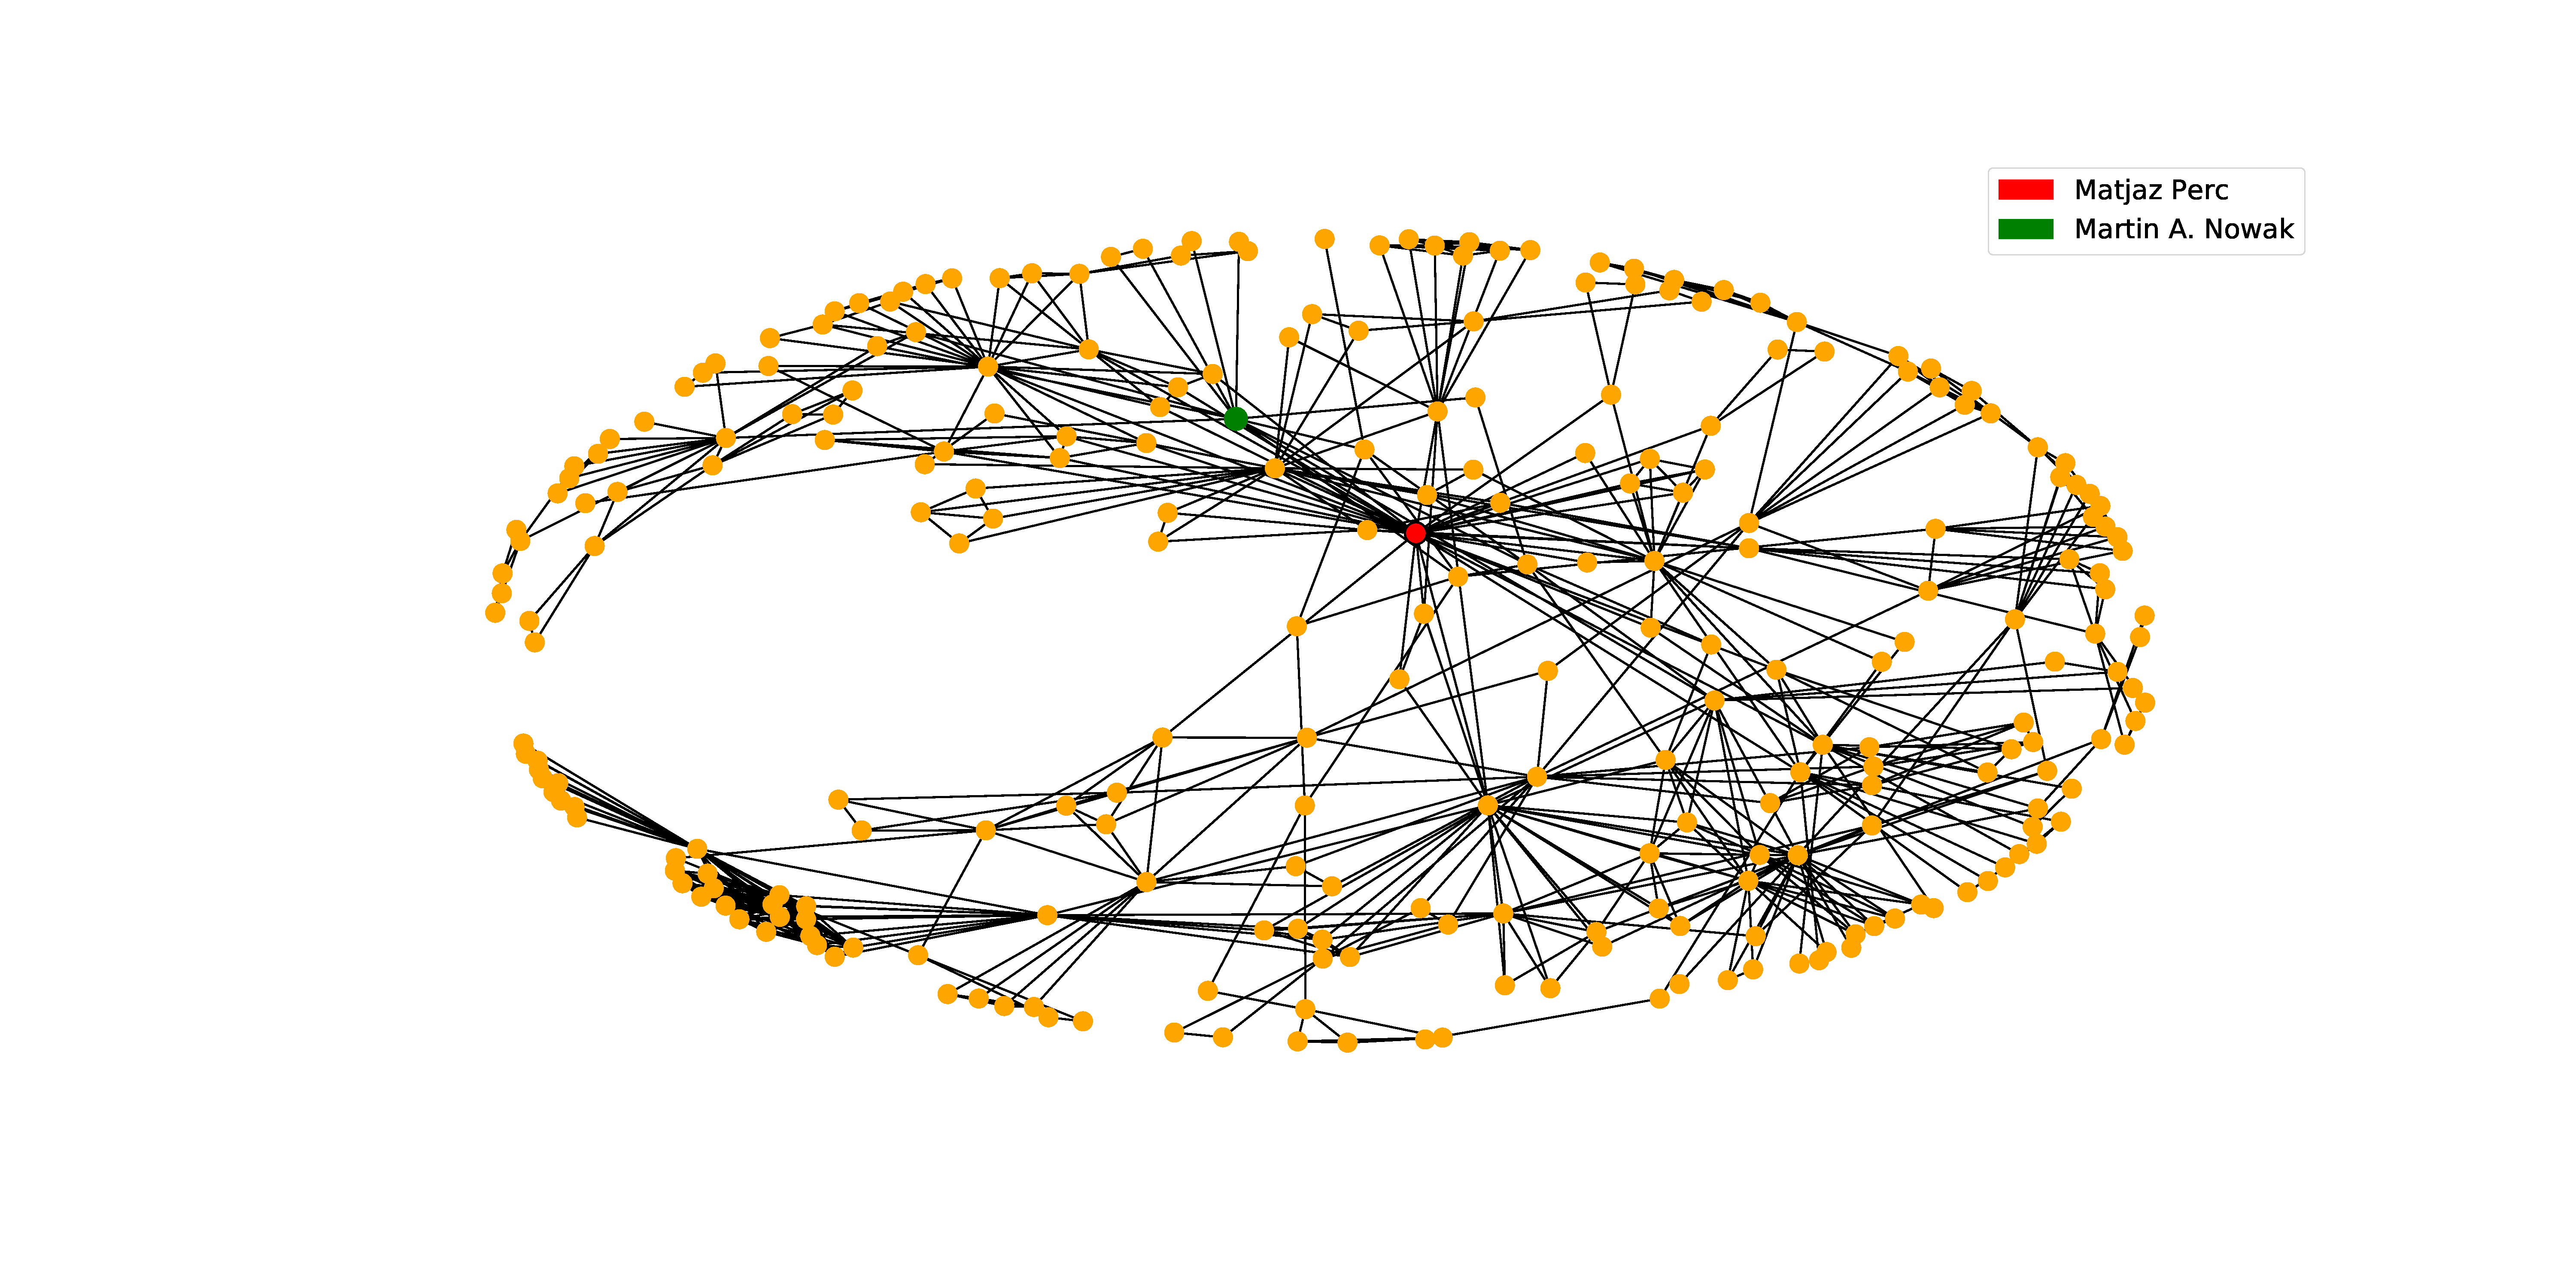
\includegraphics[width=\textwidth]{./assets/images/Perc.pdf}
    \caption{Subgraph that contains M. Nowak and M. Perc.}
    \label{fig:perc_clique}
\end{figure}

\begin{table}[!hbtp]
    \begin{center}
    \scalebox{0.8}{
    \begin{tabular}{llr}
\toprule
\(R_1\) &            Author name &  Betweenness \\
\midrule
0 &            Matjaz Perc &                0.5844 \\
1 &           Yamir Moreno &                0.4851 \\
2 &          Luo-Luo Jiang &                0.2385 \\
3 &          Arne Traulsen &                0.2164 \\
4 &        Martin A. Nowak &                0.2116 \\
5 &              V. Latora &                0.1897 \\
6 &  Krishnendu Chatterjee &                0.1441 \\
7 &          Angel Sánchez &                0.1403 \\
8 &           Han-Xin Yang &                0.1138 \\
9 &            Zhihai Rong &                0.1068 \\
\bottomrule
\end{tabular}

    \begin{tabular}{llr}
\toprule
\(R_2\) &       Author name &  Closeness \\
\midrule
0 &       Matjaz Perc &              0.3296 \\
1 &      Yamir Moreno &              0.3231 \\
2 &      Cheng-Yi Xia &              0.2886 \\
3 &     Sandro Meloni &              0.2816 \\
4 &     Alberto Aleta &              0.2789 \\
5 &     Arne Traulsen &              0.2777 \\
6 &     Angel Sánchez &              0.2746 \\
7 &     Luo-Luo Jiang &              0.2731 \\
8 &  Manfred Milinski &              0.2693 \\
9 &    José A. Cuesta &              0.2666 \\
\bottomrule
\end{tabular}

    \begin{tabular}{llr}
\toprule
\(R_3\) &            Author name &  Page rank \\
\midrule
0 &            Matjaz Perc &              0.0205 \\
1 &          Angel Sánchez &              0.0167 \\
2 &              Long Wang &              0.0156 \\
3 &              Zhen Wang &              0.0150 \\
4 &        Attila Szolnoki &              0.0134 \\
5 &  Krishnendu Chatterjee &              0.0127 \\
6 &           Yamir Moreno &              0.0121 \\
7 &           Gyorgy Szabo &              0.0112 \\
8 &           Dirk Helbing &              0.0109 \\
9 &        Martin A. Nowak &              0.0108 \\
\bottomrule
\end{tabular}
}
    \caption{Central authors based on different centrality measures of the subgraph
    which includes author M. Nowak and M. Perc.}
    \label{table:perc_clique}
    \end{center}
\end{table}

\subsection{Conclusions from the analysis}

In this section of the paper it was described how insights on the research of the
field can be gained by performing a data analysis. Initially the method that
was used to collect various metadata of articles was briefly presented.

Secondly, the number of articles and their provenance over the years was
reviewed. The number of articles appears to be gradually increasing after 2000.
That could be because most of the journals used in the data collection are either
recent or focused on computing/engineering sciences that have been used in the
field mainly after 2000.

One of the features retrieved by the collection is the authors name. Exploring
the connections of these authors has been the main focus of the section as it
provides several interesting findings.The aims of the network analysis have been,

\begin{itemize}
    \item to research how collaborative the field of the prisoner's dilemma is;
    \item indentify the most crucial authors of the network;
    \item explore several specific collaborations.
\end{itemize}

Researching the collaborative behaviour of the the field is achieved by examining
several network measures. The network was proven to be rather disjoint with a
very low density adn an average degree of 3. The median degree of authors has been
two, thus most people in the area are maninly writing with two co-authors.

In order to have an objective insights as to how collaborative the field is
two other topics were considered as separate networks. The topics have been the
price of anarchy and auction games. The results have shown that the collaboration
behaviour is very similar to all three topics. The average degreres of all networks
was close to 3 and all had a very small density. Furthermore, there was not a
significant difference between the degree distributions of the topics.

However, the historical progress of the authorship is it significant different
between the fields. Auction games have been attracting more authors and collaborations
as time progresses. The price of anarchy is a new field that attracted a large
number of authors and parternshipd after 2004. The prisoner's dilemma seems to
be a more complicated, having a sudden decrease in 1960 and a sudden increase in
1970. Those this could be due the bias that this analysis suffers, which is that only
5 journals are considered. More insights can be brought in the analysis by performing
further tests.

A surprise has been that the main author that was highlighted several times
within the analysis has been M. Perc. An author whose work was not delved into
in the literature section. A number of authors such as Perc, Moreno and
Traulsen would have not come to our attention if this analysis was not held.
Thought their work seems promising and may be of interest to people that focus
on evolutionary game theory, spatial games and social stuff.
Thus advantages of such analysis is that authors that have not previously be
considered can stand out.

Another powerful results emerges by reviewing several subgraphs of authors.
The connections to an author of interest can offer new opportunities and guidelines
as to whose work to follow next. Nevertheless, only a small number
of the subgraphs were presented here. The reader is encouraged to explore
the extra material of this work and investigate the connection of their chosen
author.

\newpage
\bibliographystyle{plain}
\bibliography{bibliography.bib}
\end{document}
